\chapter{Desenvolvemento do sistema}
\minitoc
\label{chap:implementacion}
\vspace{0.5cm}

%%%%%%%%%%%%%%%%%%%%%%%%%%%%%%%%%%%%%%%%%%%%%%%%%%%%%%%%%%%%%%%%%%%%%%%%%%%%%%%%
% Objetivo: Exponer las partes relevantes de la implementación                 %
%%%%%%%%%%%%%%%%%%%%%%%%%%%%%%%%%%%%%%%%%%%%%%%%%%%%%%%%%%%%%%%%%%%%%%%%%%%%%%%%

\lettrine{N}{este} capítulo exporase o desenvolvemento do proxecto baseándose
no esquema proporcionado pola planificación inicial: desde o deseño software e
hardware de baixo nivel do sistema ata a implementación e o ensamblado do
producto, pasando por un prototipo operacional.

\section{Determinación}

 \subsection{Obxectivos}

 Establecéronse os obxectivos da fase de desenvolvemento do proxecto. \\

 Obxectivos:

 \begin{itemize}
  \item Implementar unha gaita MIDI sen fíos en tempo real empregando
        software/hardware libre.
 \end{itemize}

 \subsection{Alternativas}

 Establecéronse posibles alternativas a eses obxectivos, aplicables no caso de
 que estes non se puidesen cumprir. \\

 Alternativas:

 \begin{itemize}
  \item Se non é posible implementar completamente o proxecto, pode optarse
        por:
        \begin{enumerate}
         \item Se é por causa de que o hardware non o permite, cambiar as pezas
               correspondentes por outras que si o permitan.
         \item Se as partes que non é posible implementar son opcionais ou de
               pouco peso, desbotalas e implementar o resto.
         \item Cancelar e mudar de proxecto.
        \end{enumerate}
 \end{itemize}

 \subsection{Restriccións}

 Establecéronse restriccións aplicables a ditos obxectivos.

 \begin{enumerate}
  \item As propias restriccións veñen dadas polo propio título do proxecto. A
        saber:
        \begin{enumerate}
         \item Empregar o protocolo MIDI.
         \item Empregar tecnoloxía sen fíos.
         \item Empregar tempo real.
         \item Empregar software libre.
         \item Empregar harwdware libre.
         \item E/ou as derivadas de calquera das súas alternativas.
        \end{enumerate}
 \end{enumerate}

\section{Avaliación de alternativas e resolución de riscos}

 \subsection{Análise de riscos}

 Determináronse os riscos que comportaban as distintas alternativas e as súas
 posibles solucións.

 \begin{enumerate}
  \item Alternativas 1.
        \begin{enumerate}
         \item Riscos:
               \begin{enumerate}
                \item Que non exista hardware alternativo que soporte a
                      implemtación das características restantes.
                \item Que as partes a desbotar sexan partes importantes ou
                      incluso críticas.
                \item Que o tempo restante para a execución do proxecto non
                      sexa suficiente.
               \end{enumerate}
         \item Solucións:
               \begin{enumerate}
                \item Recortar características ou cancelar e mudar de proxecto.
                \item Aplicar medidas de mitigación para que a planificación
                      non se vexa afectada en extremo, ou cancelar e mudar de
                      proxecto se fan inviable o mesmo.
                \item Agardar a presentalo na seguinte convocatoria.
               \end{enumerate}
        \end{enumerate}
 \end{enumerate}

 \subsection{Prototipo operacional}
 
 Nesta fase desenvolveuse o seguinte nivel de prototipado, tanto hardware coma
 software, sendo xa ambos operacionais. \\
 
 A aproximación seguida foi aplicar \textit{BDD} \cite{BDD} ou \textit{TDD}
 \cite{TDD} segundo o caso, en dirección \textit{top-dowm} obtendo así as
 sinaturas dos servizos e o comportamento desexado dos mesmos primeiro, para
 logo facer unha implementación \textit{bottom-up} respectando o deseño
 conseguido previamente.

  \subsubsection{Prototipo hardware}
  
  Para a o prototipo hardware operacional tiramos do prototipo deseñado na fase
  anterior, para o cal empregamos ferramentas CAD co fin de poder facer probas
  en formato dixital antes de pasar a formato físico, evitando así os múltiples
  problemas relacionados.

   \paragraph{Integración do hardware}
   
   Unha vez claro o deseño sobre o papel, montouse un prototipo físico con cada
   compoñente por separado, de maneira que inicialmente se puidera probar cada
   un de maneira unitaria, antes de pasar á integración final. \\
   
   Desta maneira, dividiuse a montaxe completa en varias submontaxes:
   
   \begin{itemize}
    \item Router (figura \ref{figura:Router}).
    \item Receptor (figura \ref{figura:Receptor}).
    \item Sensor de presión (figura \ref{figura:SensorPresion}).
    \item Sensores capacitivos (figura \ref{figura:SensoresCapacitivos}).
    \item Lector de tarxetas (figura \ref{figura:LectorTarxetas}).
   \end{itemize}
   
   A primeira montaxe foi a do router por resultar a máis sinxela, xa que
   consistiu nunha placa Arduino Uno sobre a que se montou unha placa auxiliar
   onde se montou o transmisor XBee, todo sen maior problema por ser altamente
   acoplables, sendo logo embebidos nunha caixa a medida e conectados por USB
   ó ordenador onde se executa a aplicación de configuración e o servidor
   MIDI. \\
   
   A nivel de sinatura de servizos, ó funcionar coma un simple router
   automatizado, non tiña máis que probar a transmisión correcta de datos, que
   decidiu deixarse coma último punto da integración hardware por razóns de
   fiabilidade na transmisión dos mesmos. \\
   
   \begin{figure}[htbp]
    \centering
    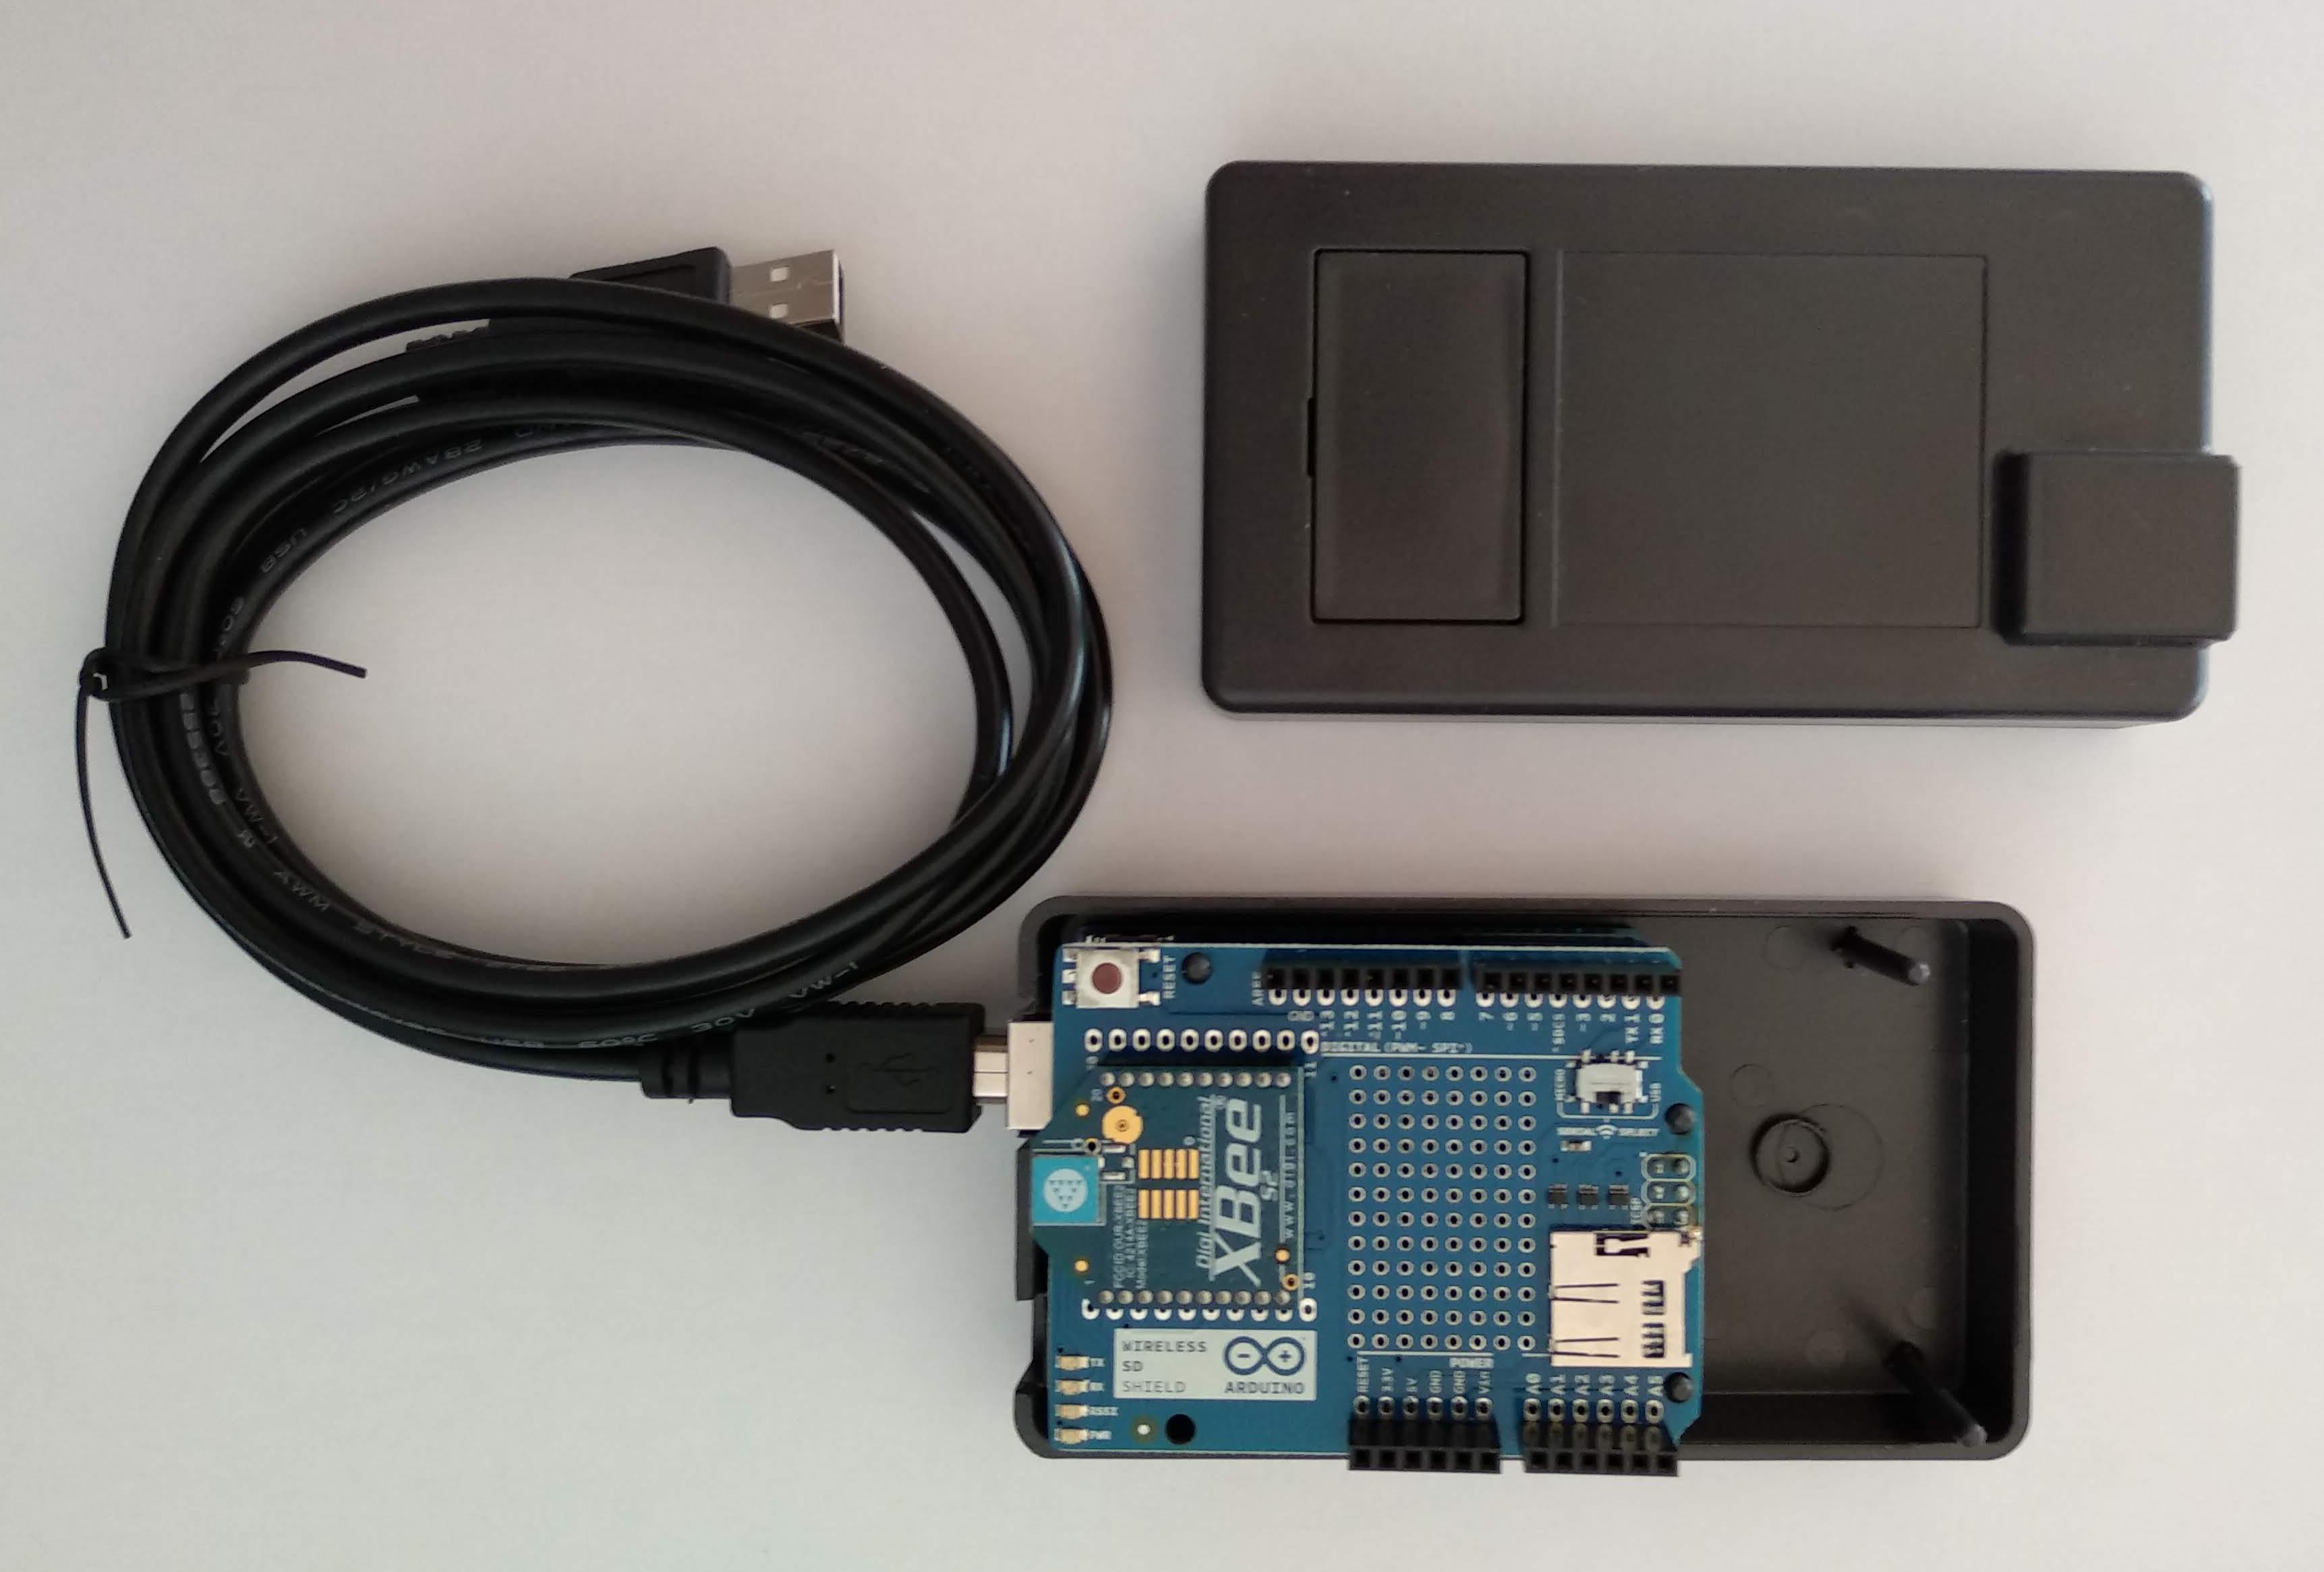
\includegraphics[scale=0.15,keepaspectratio=true]{./imagenes/router.jpg}
    % router.jpg: 640x480 pixel, 72dpi, 22.58x16.93 cm, bb=0 0 640 480
    \caption{Router}
    \label{figura:Router}
   \end{figure}
   
   A seguinte montaxe foi a do receptor, moi similar á do router, pois non deixa
   de ser unha placa Arduino Fio, que xa dispón dun zócalo para o módulo XBee e
   polo que non precisa de placa auxiliar. \\
   
   Polo mesmo motivo que o anterior, deixouse para máis adiante coma o último
   punto ou nivel de integración, pois resulta máis robusto probar e medir
   primeiro de maneira cableada e logo pasar ó modo sen fíos e poder comparar
   medicións e resultados. \\
  
   \begin{figure}[htbp]
    \centering
    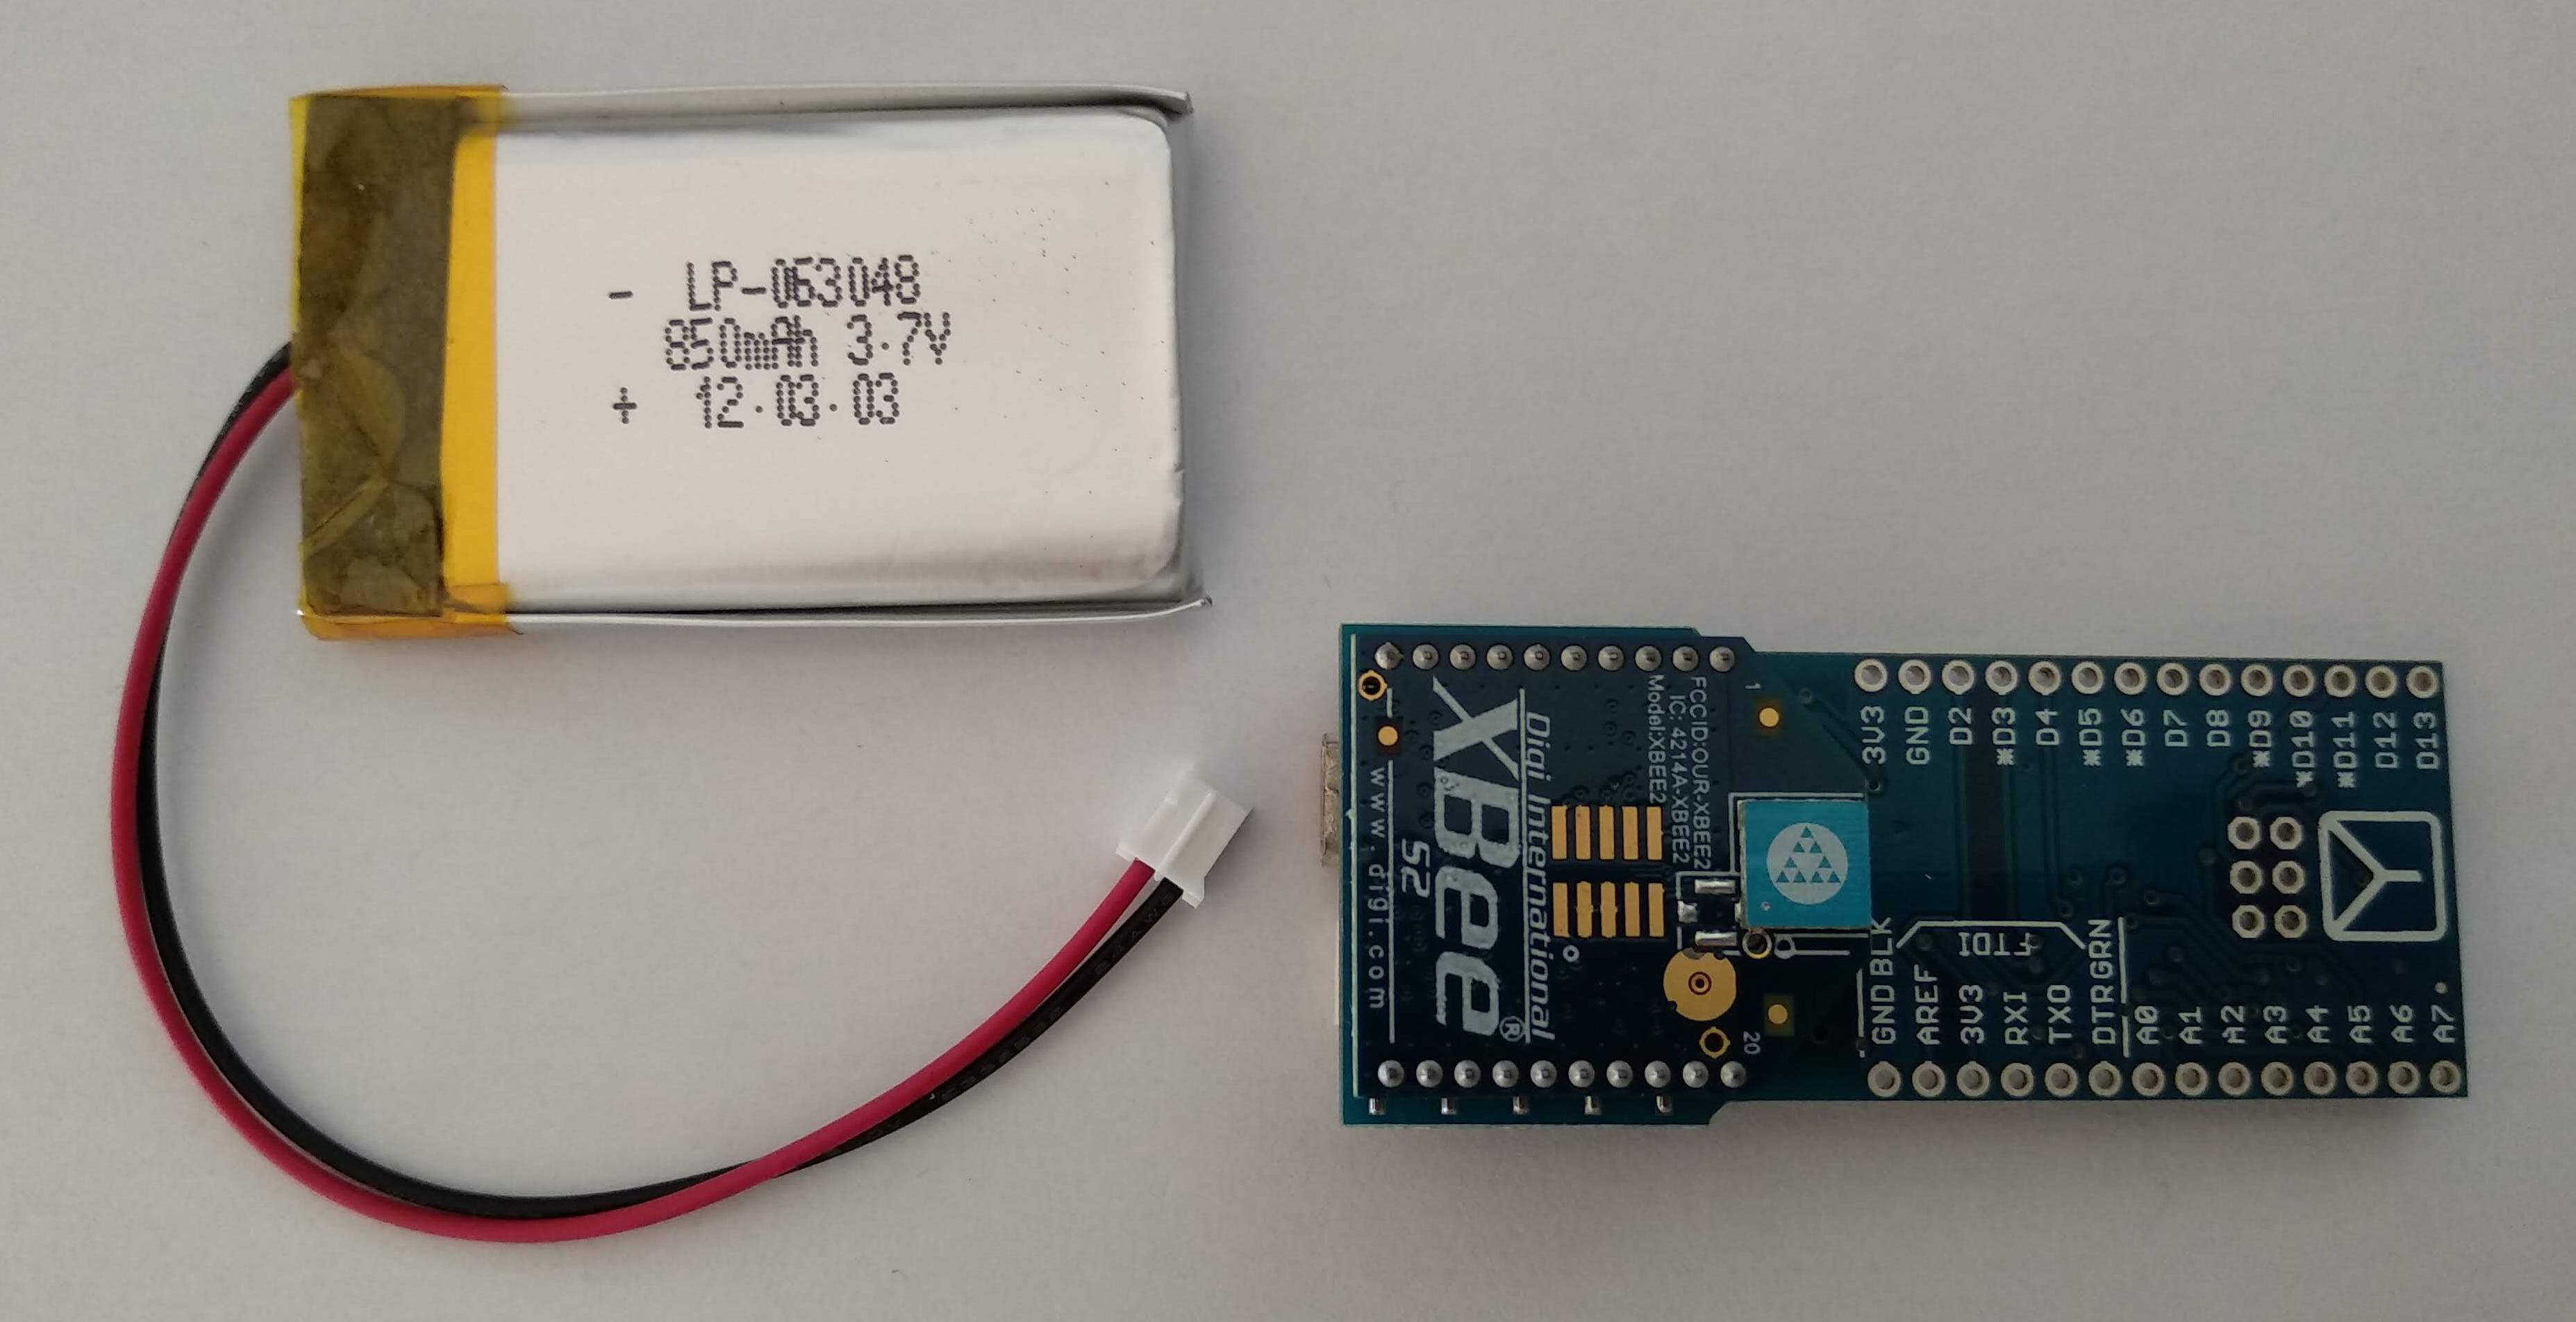
\includegraphics[scale=0.15,keepaspectratio=true]{./imagenes/receptor.jpg}
    % receptor.jpg: 640x480 pixel, 72dpi, 22.58x16.93 cm, bb=0 0 640 480
    \caption{Receptor}
    \label{figura:Receptor}
   \end{figure}
   
   No seu lugar, para desenvolver a lóxica de negocio da gaita MIDI, empregouse
   unha placa Arduino Uno, que conta coas mesmas características, salvo pola
   conexión directa do módulo XBee e que conta coa vantaxe de que podemos
   descargar nela o firmware da nosa implementación directamente a través dun
   cable USB. \\
   
   Neste caso a interface pública veu definida polo propio funcionamento de
   Arduino, contando cun método de configuración inicial e outro de execución
   continua. \\
   
   O que fixemos neste caso foi facer unha primeira implementación en
   pseudo-código do comportamento xeral que tería o dispositivo, intentando
   ver a qué periférico tería que chamar en cada caso, cándo e cómo, dando como
   resultado dúas partes claramente diferenciadas:
   
   \begin{itemize}
    \item Configuración das características propias da gaita.
    \item E reproducción ou envío de mensaxes MIDI.
   \end{itemize}
   
   Na parte de configuración, realizaríase tanto a carga dos parámetros
   configurables ó inicio coma o intercambio de configuracións entre o
   dispositivo e a aplicación de configuración, para o que sería preciso tirar
   do lector de tarxetas para persistir a información, así coma unha librería
   JSON para darlle formato un formato usable á mesma e da que falaremos máis
   adiante. \\
   
   En canto á parte de reproducción, sería preciso avaliar a presión do fol para
   decidir se o dispositivo debe soar ou non e a dixitación actual a través dos
   sensores capacitivos para ver se corresponde con algunha válida e por tanto
   producir o son relativo á mesma mediante o emprego dunha librería MIDI da que
   tamén falaremos máis adiante. \\
   
   Ampliaremos esta lóxica polo miúdo cando cheguemos á parte software, facendo
   uso de diagramas de fluxo. \\
   
   A continuación procedeuse co sensor de presión, por ser o seguinte máis
   sinxelo en orde de funcionalidade, pois o único que precisamos obter del é a
   presión dentro do fol, aínda que pode devolver máis parámetros relacionados
   coa mesma. \\
   
   Como se pode ver na imaxe, conectouse a unha placa Arduino Uno empregando
   o bus I2C do mesmo. \\
  
   \begin{figure}[htbp]
    \centering
    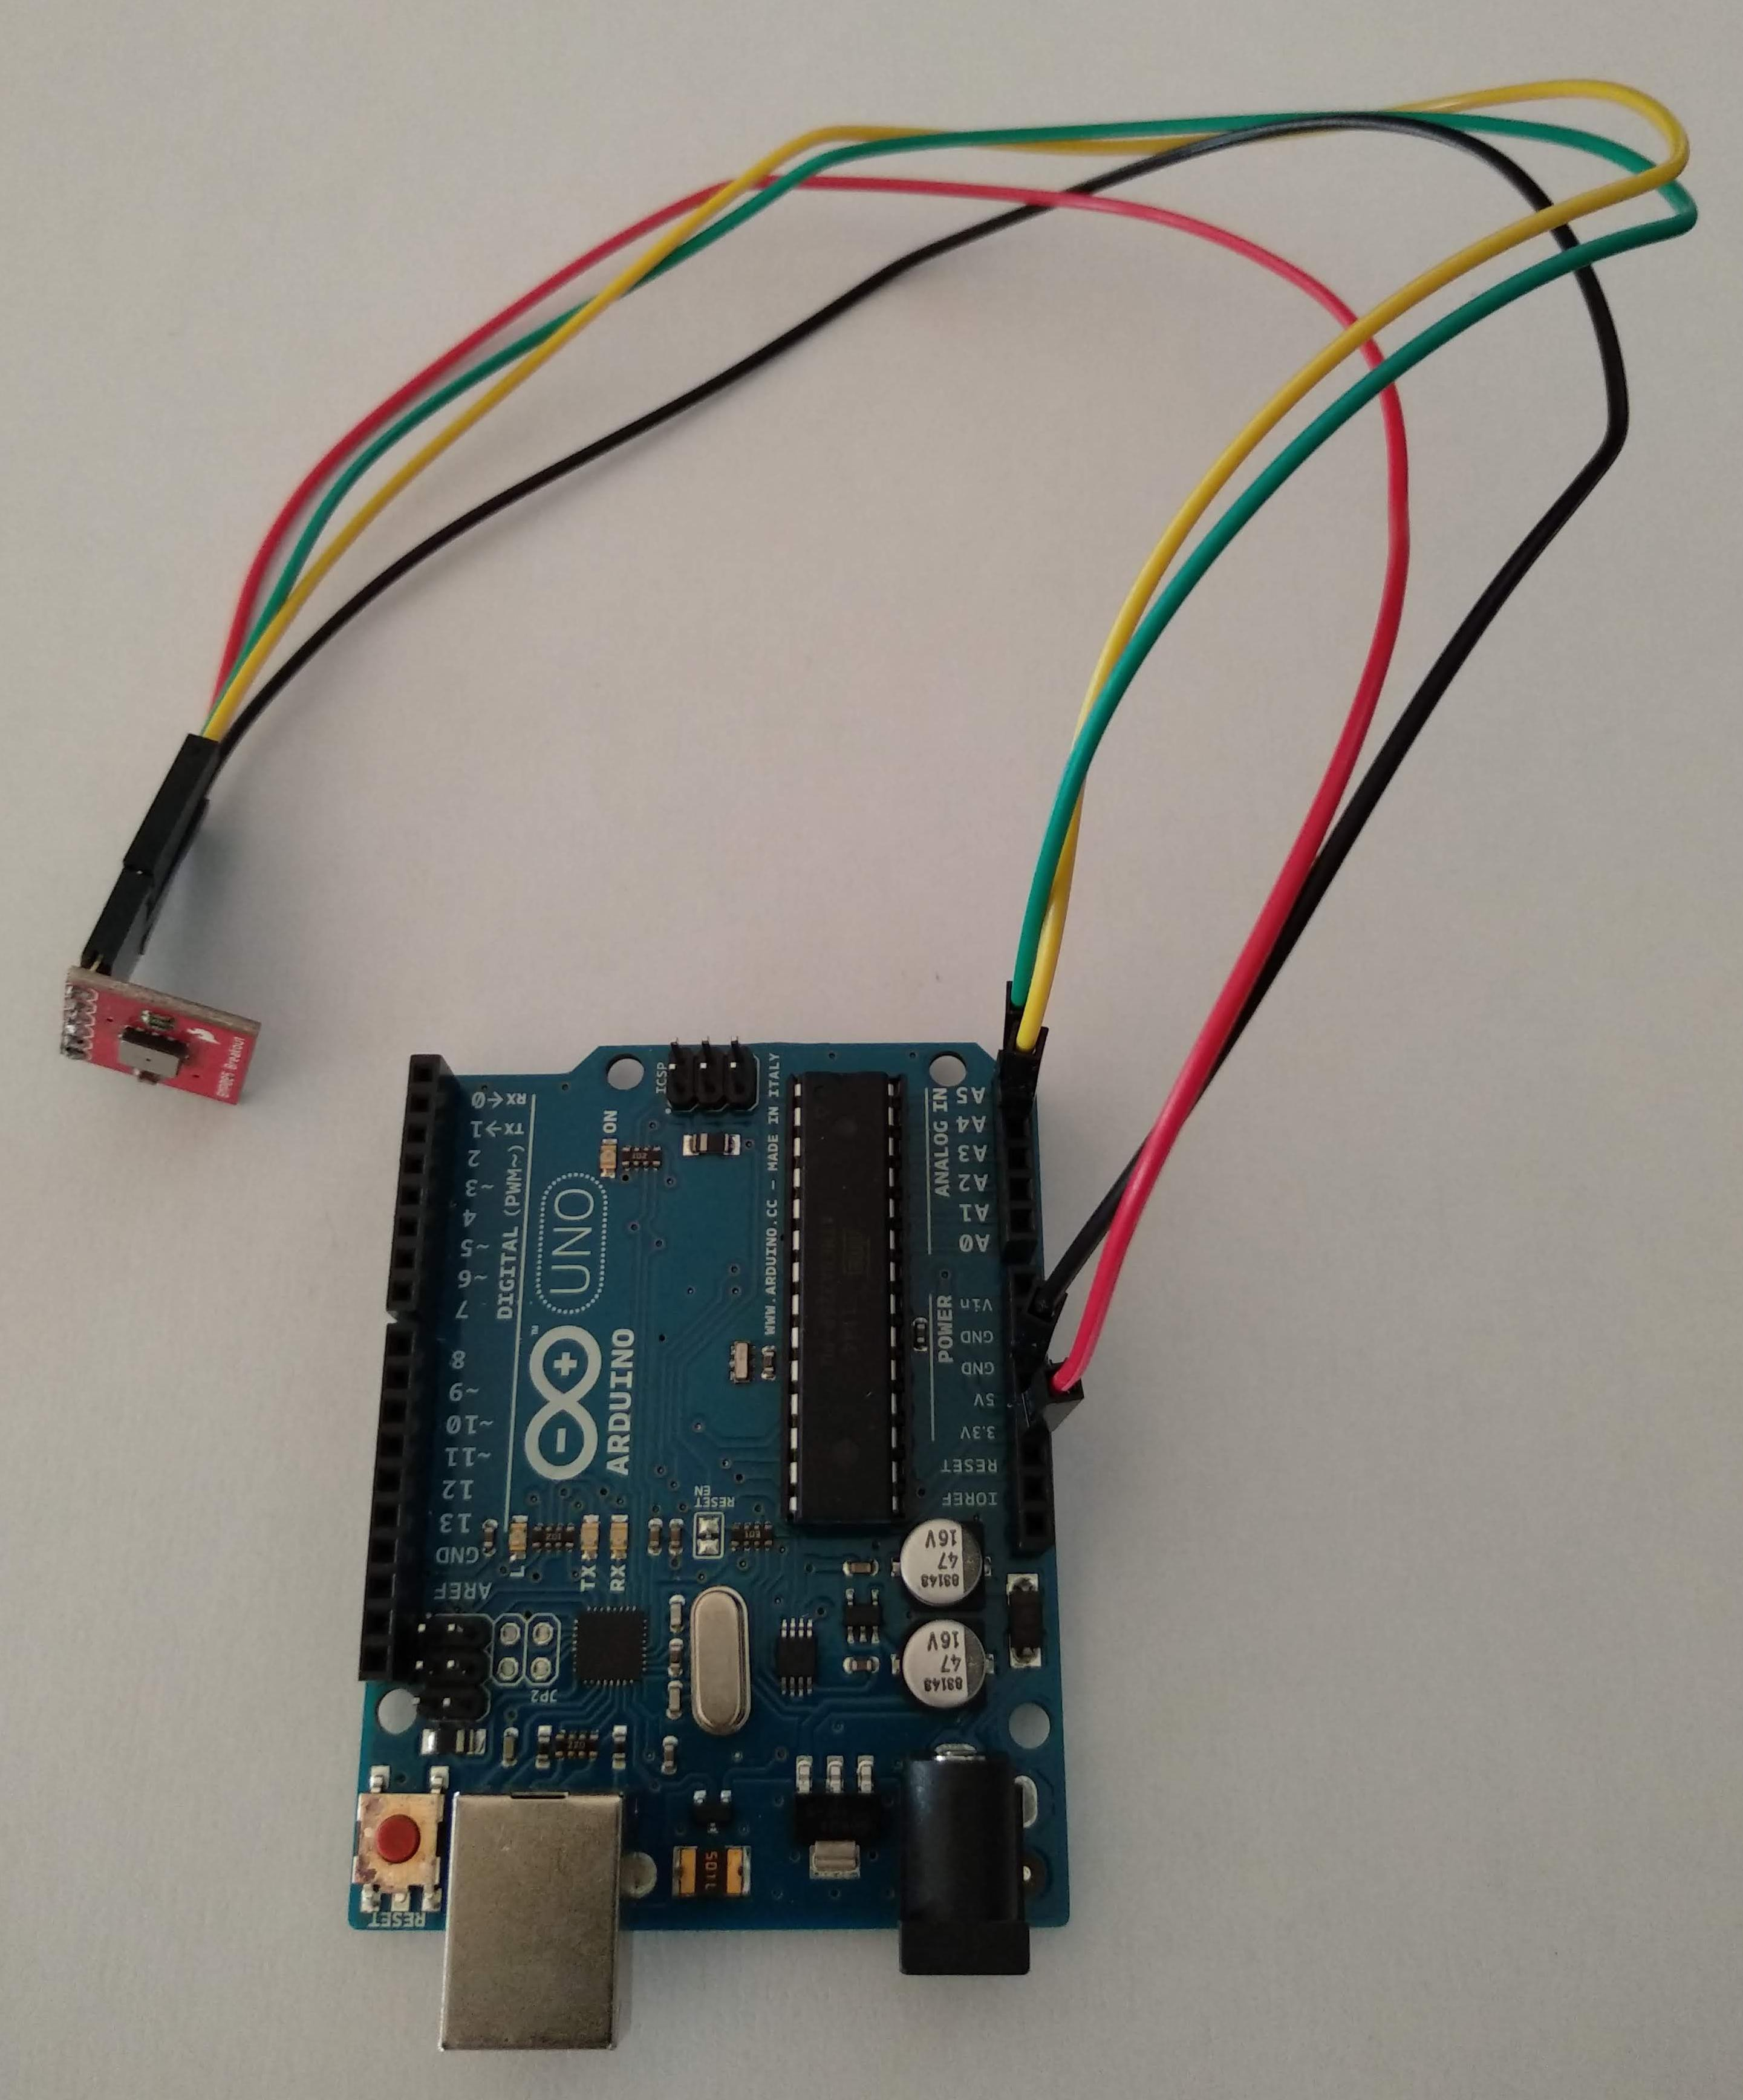
\includegraphics[scale=0.2,keepaspectratio=true]{./imagenes/sensor-presion.jpg}
    % sensor-presion.jpg: 640x480 pixel, 72dpi, 22.58x16.93 cm, bb=0 0 640 480
    \caption{Sensor de presión}
    \label{figura:SensorPresion}
   \end{figure}
   
   Ademáis de definir a súa interface pública (figura 
   \ref{figura:InterfaceSensorPresion}) para a obtención da presión e un
   ficheiro de proba (figura \ref{figura:TestSensorPresion}) para validar a
   implementación completa posterior. \\
   
   \begin{figure}[htbp]
    \centering
    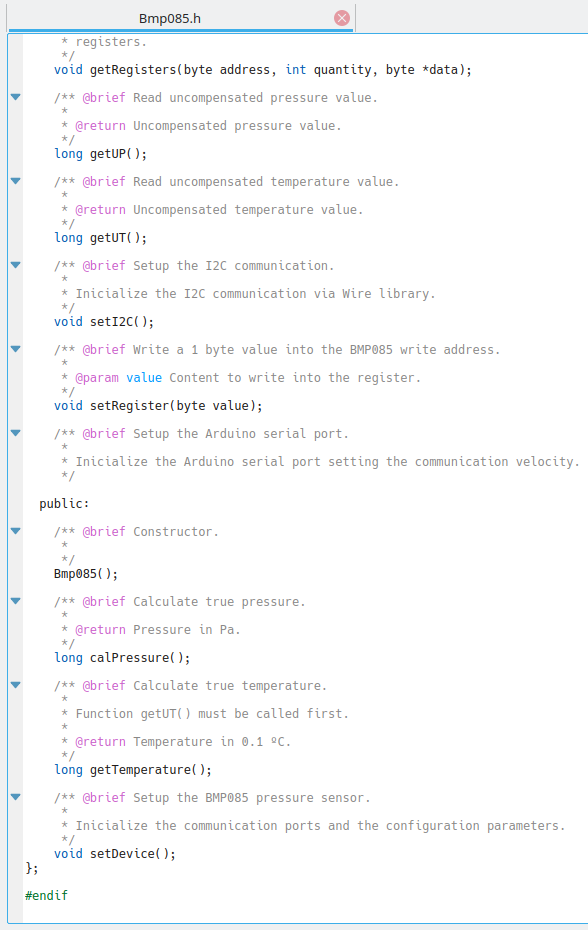
\includegraphics[scale=0.8,keepaspectratio=true]{./imagenes/interface-sensor-presion.png}
    % interface-sensor-presion.png: 640x480 pixel, 72dpi, 22.58x16.93 cm, bb=0 0 640 480
    \caption{Interface do sensor de presión}
    \label{figura:InterfaceSensorPresion}
   \end{figure}
   
   \begin{figure}[htbp]
    \centering
    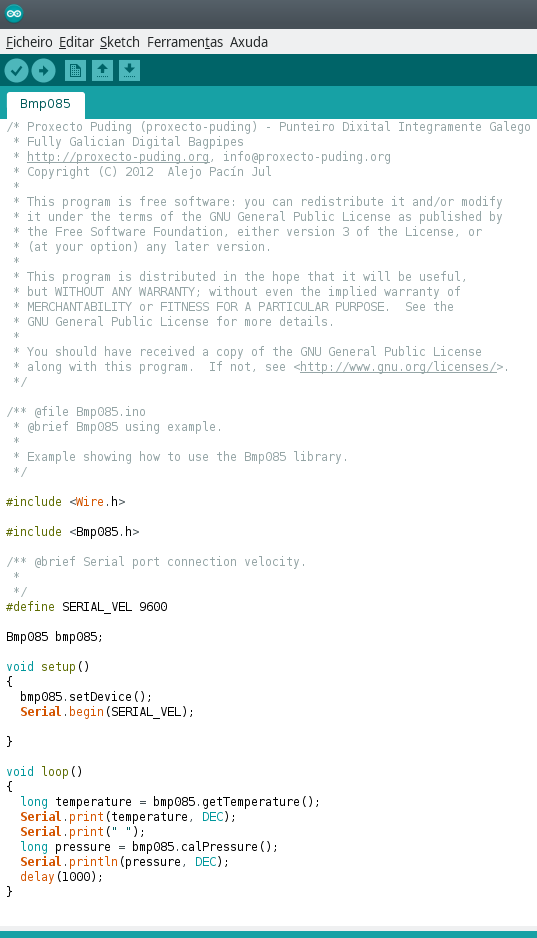
\includegraphics[scale=0.8,keepaspectratio=true]{./imagenes/test-sensor-presion.png}
    % test-sensor-presion.png: 640x480 pixel, 72dpi, 22.58x16.93 cm, bb=0 0 640 480
    \caption{Ficheiro de proba do sensor de presión}
    \label{figura:TestSensorPresion}
   \end{figure}
   
   O turno seguinte foi para os sensores capacitivos. Neste caso, o que
   precisamos saber é cáles están acesos en cada momento, de maneira que
   poidamos facer \textit{pattern matching} contra a configuración da gaita e
   saber se teriamos algún son asociado a dita dixitación, para posteriormente
   reproducilo. \\
   
   Como se pode ver na imaxe, conectouse a unha placa Arduino Uno empregando
   o bus I2C do mesmo. \\
  
   \begin{figure}[htbp]
    \centering
    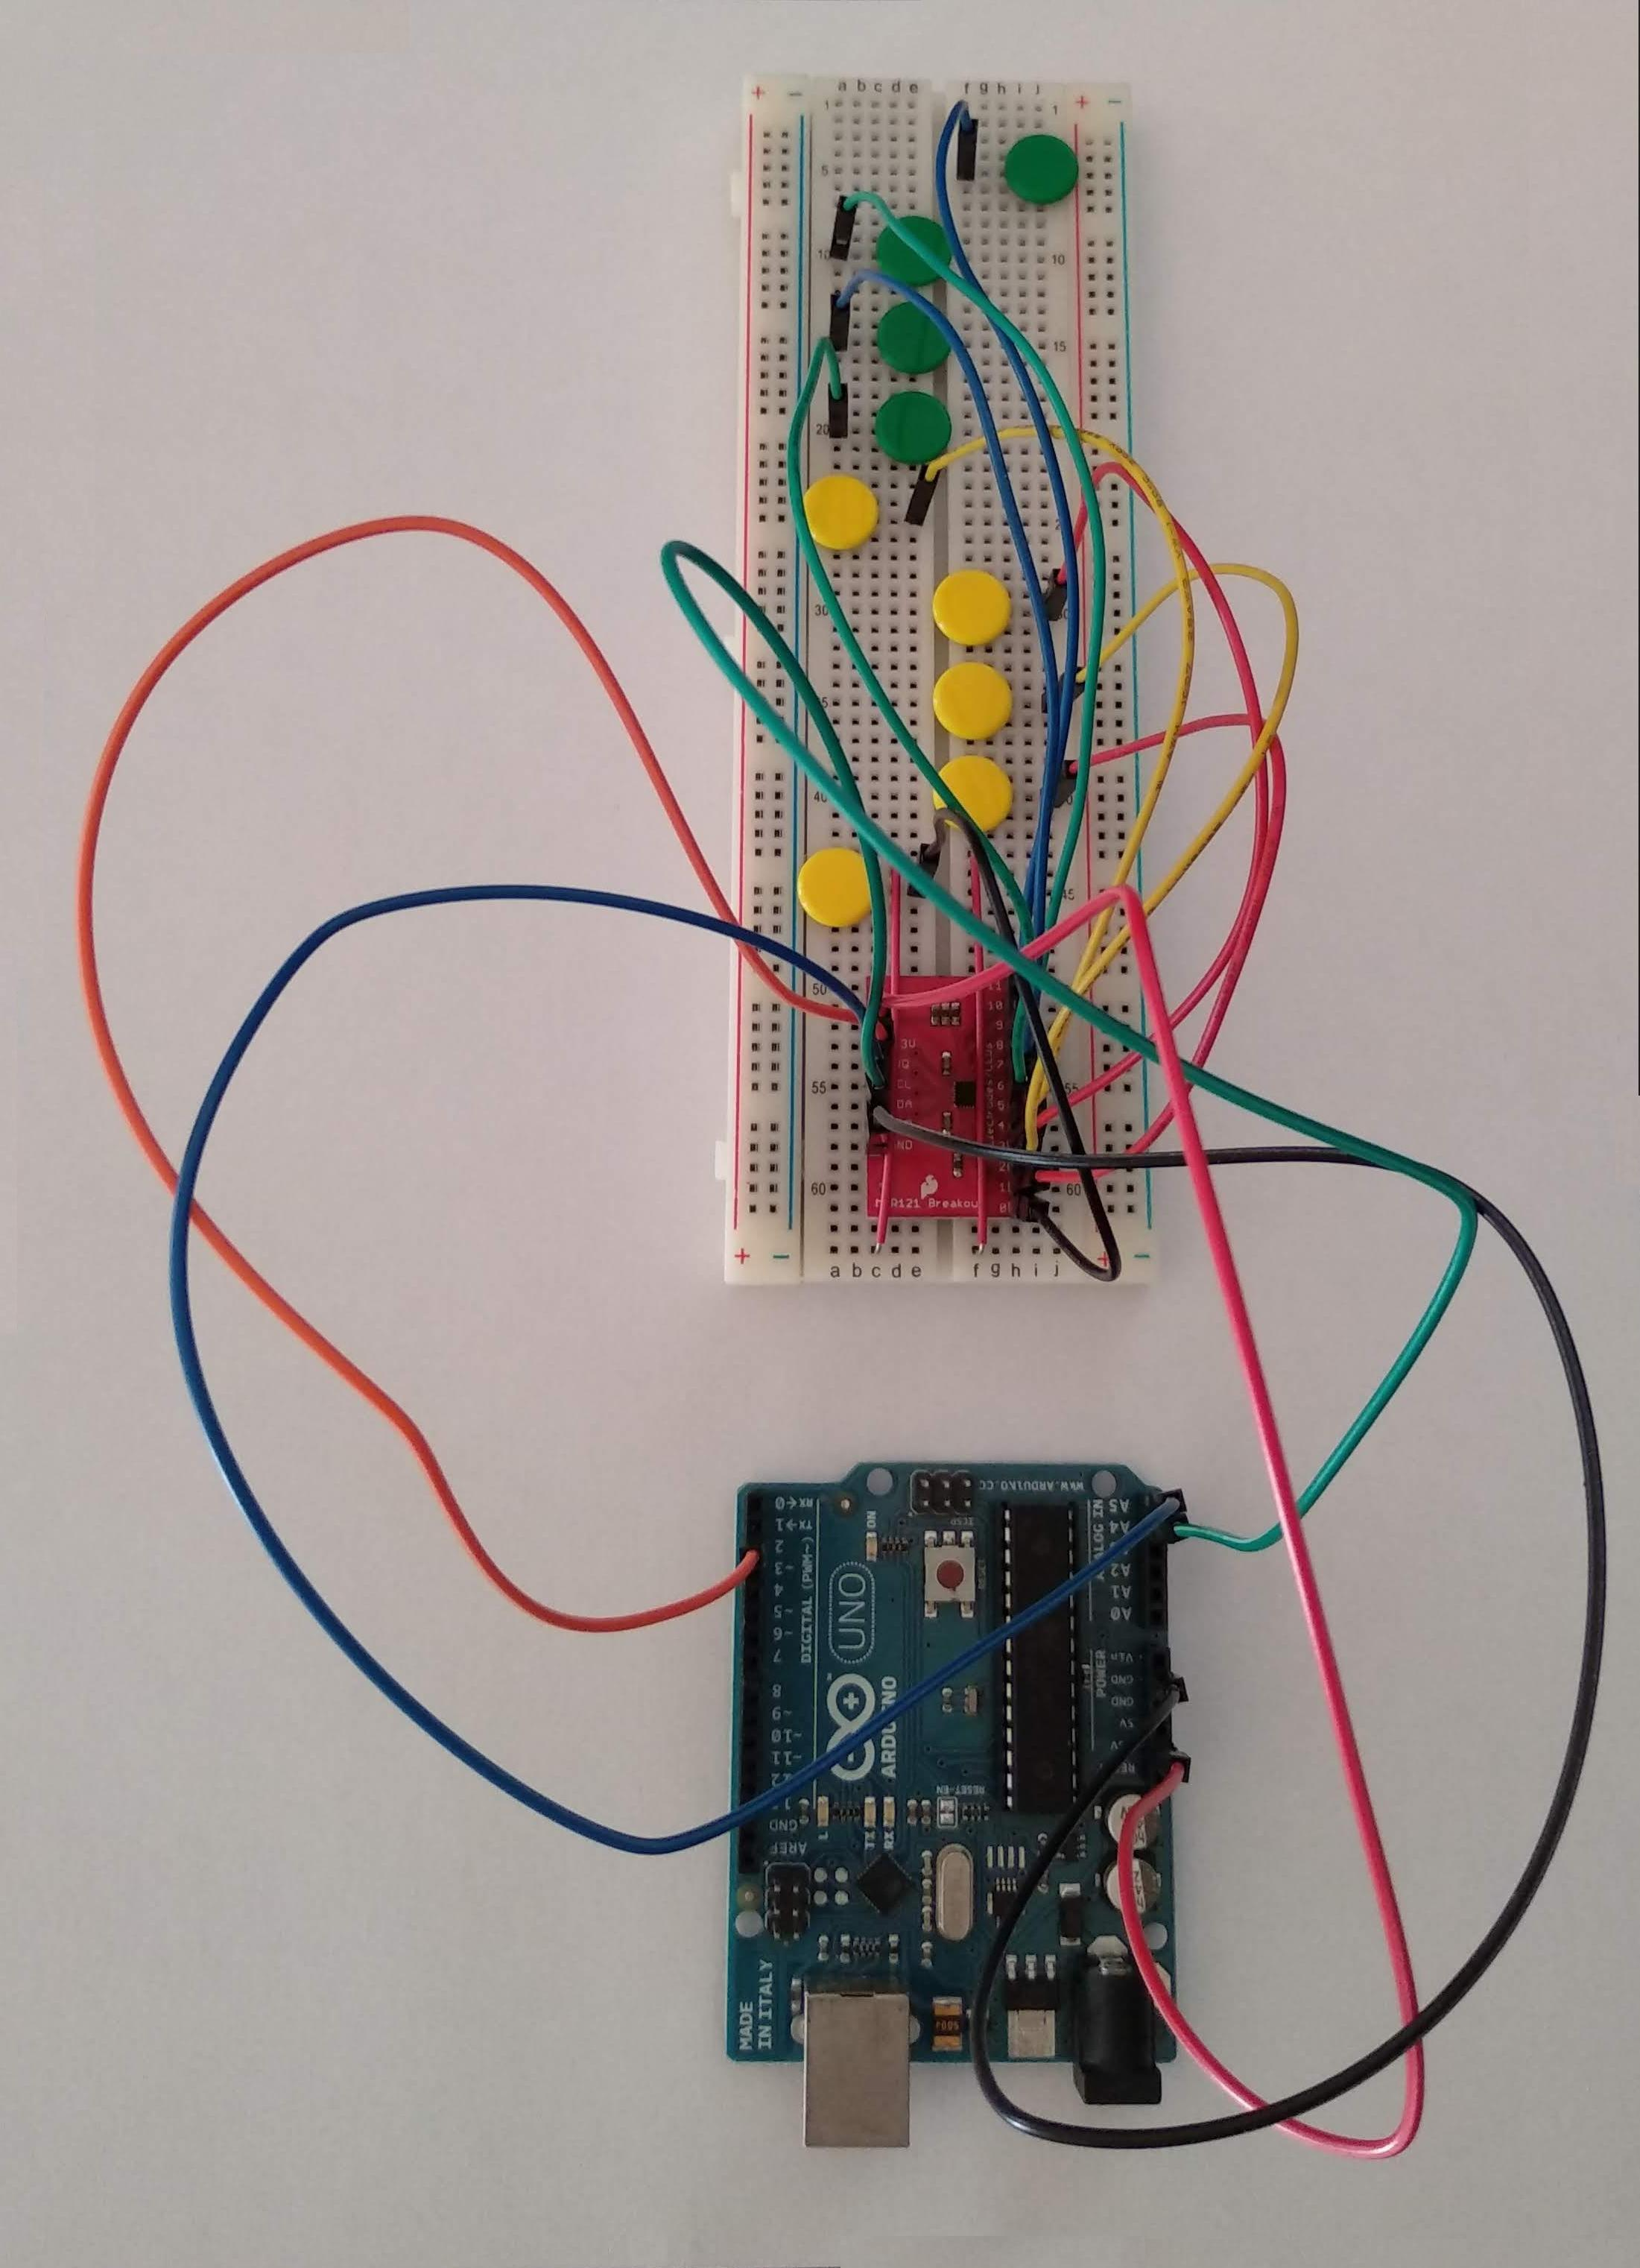
\includegraphics[scale=0.2,keepaspectratio=true]{./imagenes/sensores-capacitivos.jpg}
    % sensores-capacitivos.jpg: 640x480 pixel, 72dpi, 22.58x16.93 cm, bb=0 0 640 480
    \caption{Sensores capacitivos}
    \label{figura:SensoresCapacitivos}
   \end{figure}
   
   Ademáis de definir a súa interface pública (figura 
   \ref{figura:InterfaceSensoresCapacitivos}) para a obtención da dixitación e
   un ficheiro de proba (figura \ref{figura:TestSensoresCapacitivos}) para
   validar a implementación completa posterior. \\
   
   \begin{figure}[htbp]
    \centering
    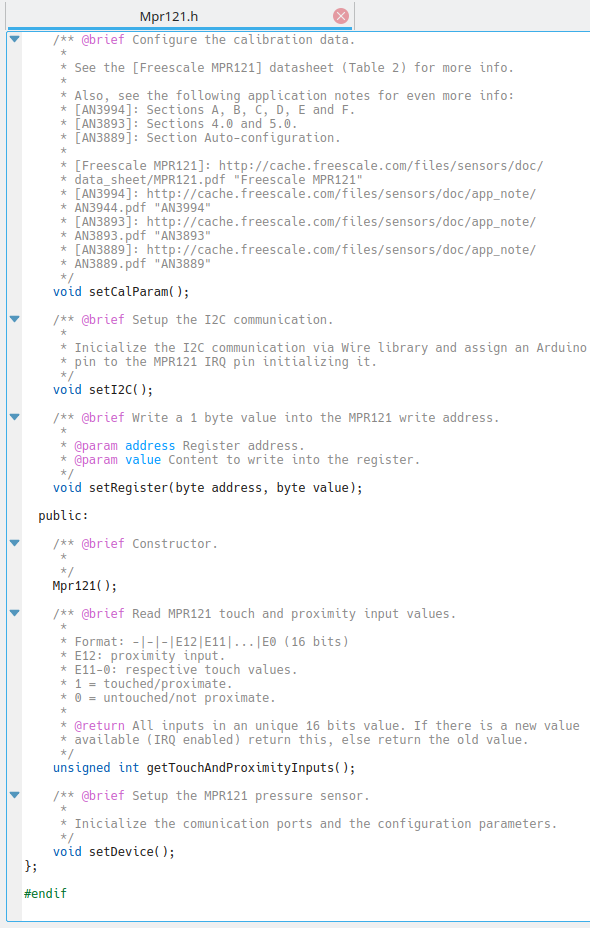
\includegraphics[scale=0.8,keepaspectratio=true]{./imagenes/interface-sensores-capacitivos.png}
    % interface-sensores-capacitivos.png: 640x480 pixel, 72dpi, 22.58x16.93 cm, bb=0 0 640 480
    \caption{Interface dos sensores capacitivos}
    \label{figura:InterfaceSensoresCapacitivos}
   \end{figure}
   
   \begin{figure}[htbp]
    \centering
    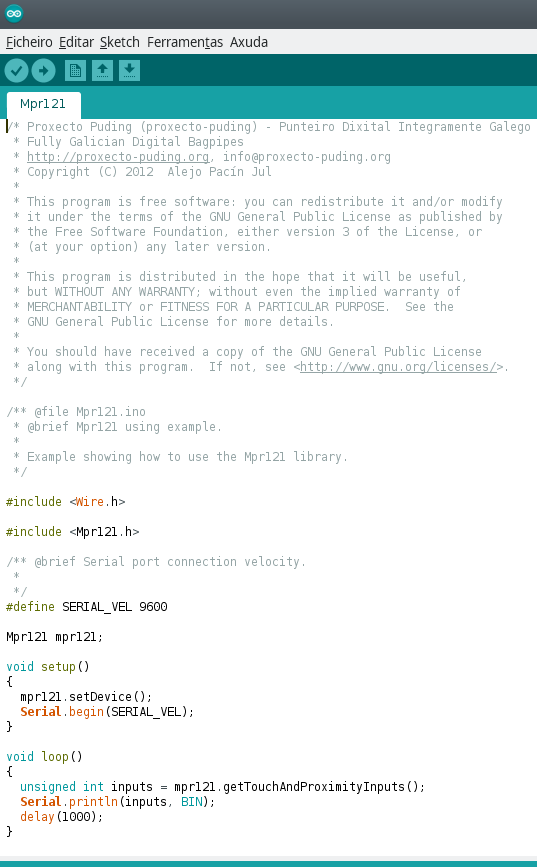
\includegraphics[scale=0.8,keepaspectratio=true]{./imagenes/test-sensores-capacitivos.png}
    % test-sensores-capacitivos.png: 640x480 pixel, 72dpi, 22.58x16.93 cm, bb=0 0 640 480
    \caption{Ficheiro de proba dos sensores capacitivos}
    \label{figura:TestSensoresCapacitivos}
   \end{figure}
   
   Para rematar cos periféricos, procedeuse co lector de tarxetas. Neste caso o
   que precisamos é poder ler e almacenar a configuración variable do
   dispositivo, de maneira que sexa independente e única para cada un dos
   mesmos. \\
   
   Como se pode ver na imaxe, conectouse a unha placa Arduino Uno empregando
   o porto UART do mesmo. \\
  
   \begin{figure}[htbp]
    \centering
    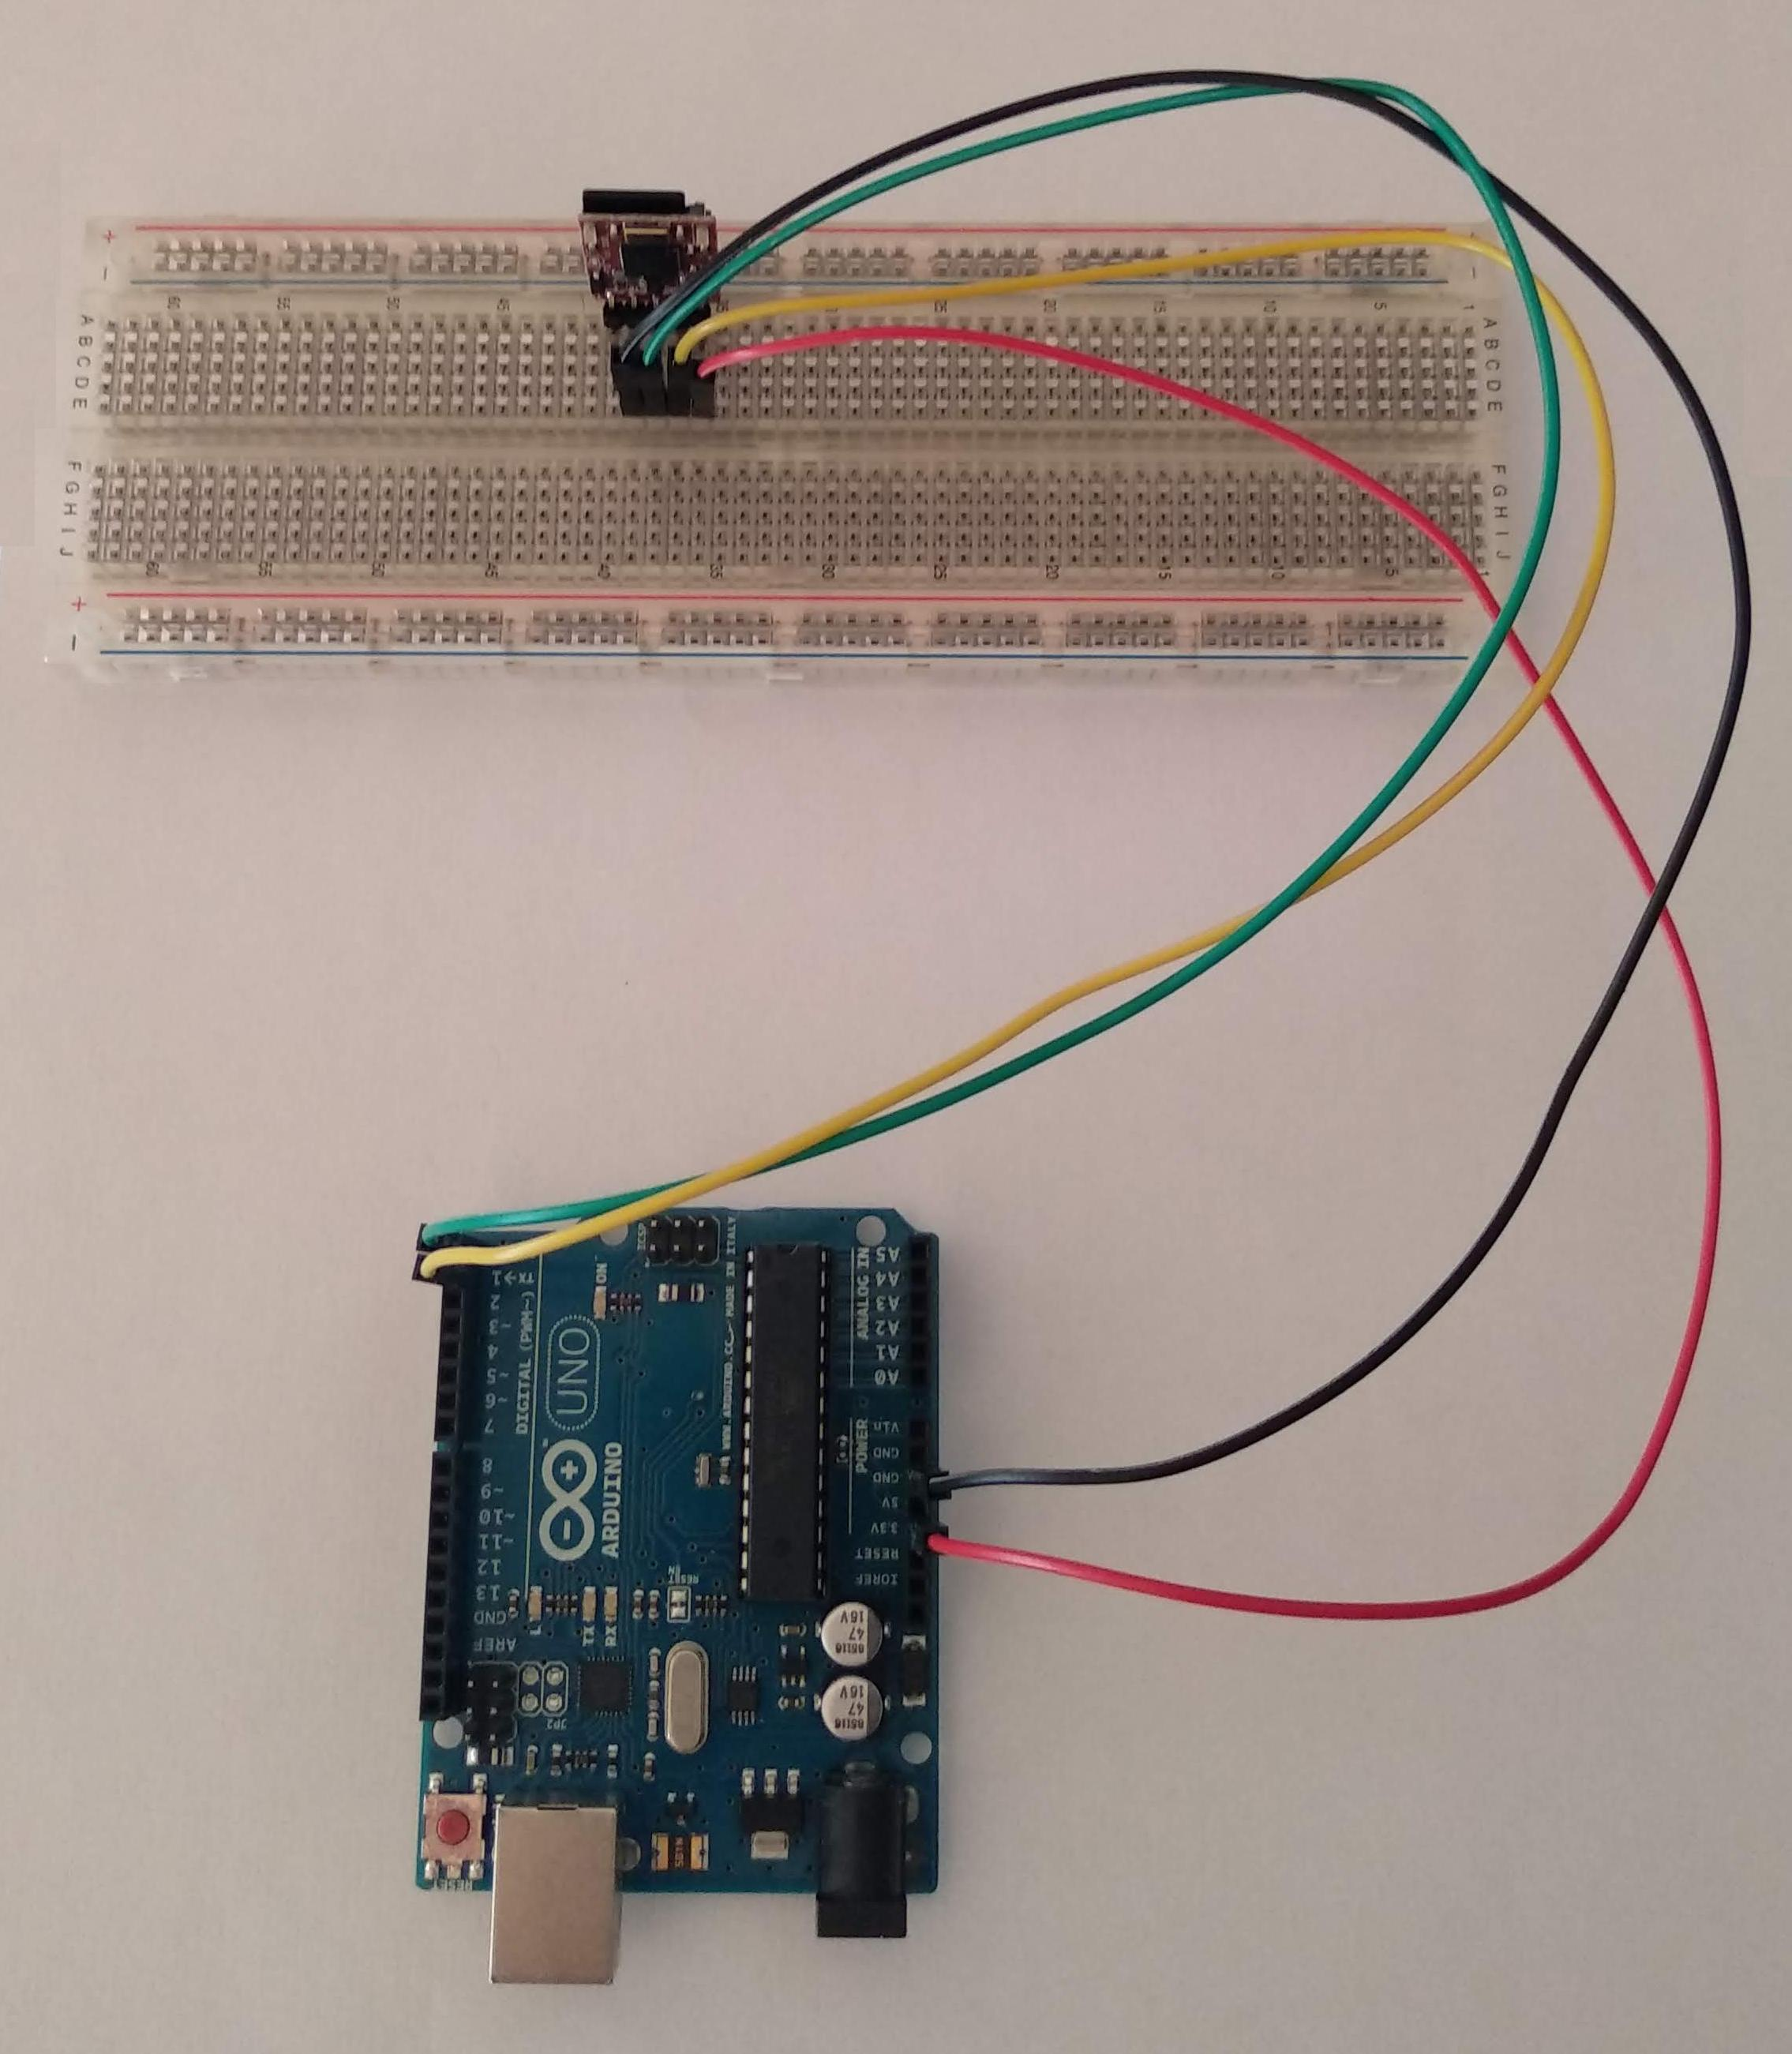
\includegraphics[scale=0.2,keepaspectratio=true]{./imagenes/lector-tarxetas.jpg}
    % lector-tarxetas.jpg: 640x480 pixel, 72dpi, 22.58x16.93 cm, bb=0 0 640 480
    \caption{Lector de tarxetas}
    \label{figura:LectorTarxetas}
   \end{figure}
   
   Ademáis de definir a súa interface pública (figura 
   \ref{figura:InterfaceLectorTarxetas}) para a obtención da configuración e un
   ficheiro de proba (figura \ref{figura:TestLectorTarxetas}) para validar a
   implementación completa posterior. \\
   
   \begin{figure}[htbp]
    \centering
    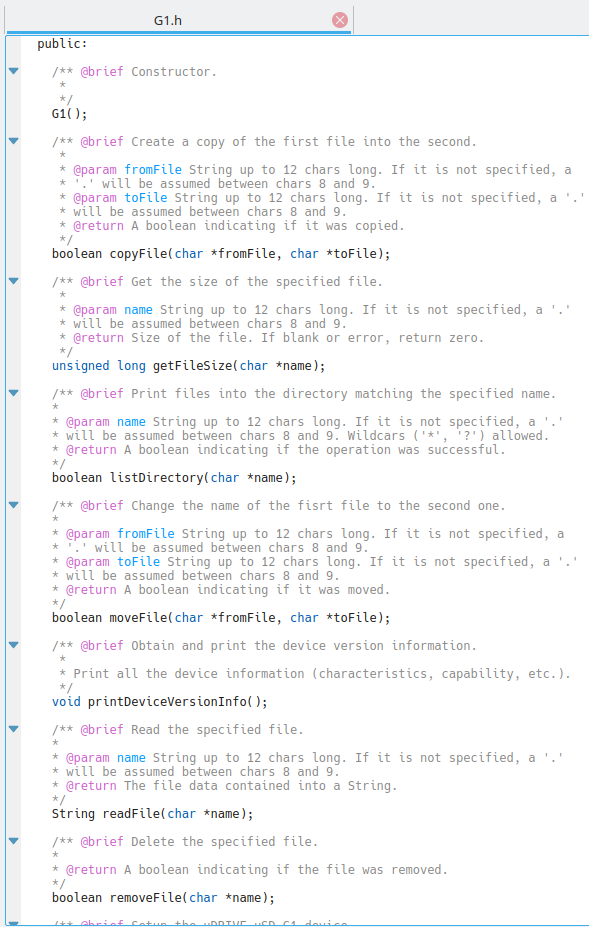
\includegraphics[scale=0.8,keepaspectratio=true]{./imagenes/interface-lector-tarxetas.png}
    % interface-lector-tarxetas.png: 640x480 pixel, 72dpi, 22.58x16.93 cm, bb=0 0 640 480
    \caption{Interface do lector de tarxetas}
    \label{figura:InterfaceLectorTarxetas}
   \end{figure}
   
   \begin{figure}[htbp]
    \centering
    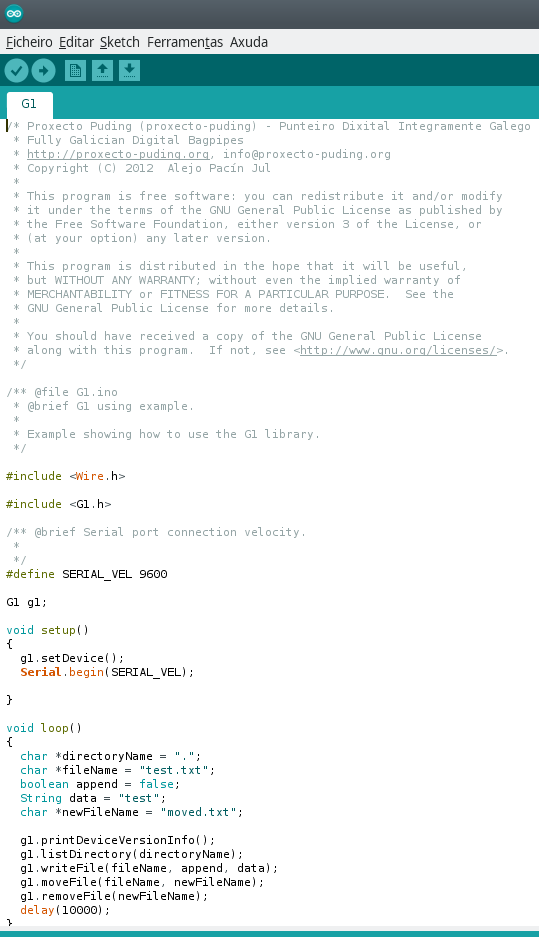
\includegraphics[scale=0.8,keepaspectratio=true]{./imagenes/test-lector-tarxetas.png}
    % test-lector-tarxetas.png: 640x480 pixel, 72dpi, 22.58x16.93 cm, bb=0 0 640 480
    \caption{Ficheiro de proba do lector de tarxetas}
    \label{figura:TestLectorTarxetas}
   \end{figure}

   \paragraph{Encapsulamento do hardware}
   
   Debido a atoparse nunha situación temperá do prototipado físico, o
   encapsulamento do hardware realizouse da maneira máis leve posible, dada a
   necesidade de poder montar e desmontar a vontade durante as probas. \\
   
   Como pode comprobarse nas imaxes do apartado anterior, o único elemento
   encapsulado por completo sería o router e o resto estaría ó aire, facendo uso
   de cables de prototipado para evitar ter que soldar e desoldar durante as
   probas. \\
   
   Ademáis, cada un dos periféricos foi montado por separado ata a integración
   completa do hardware, logo da correcta implementación, verificación e
   validación do mesmo.

  \subsubsection{Prototipo software}
  
  Para a o prototipo software operacional tiramos do prototipo deseñado na fase
  anterior e dos diagramas UML relacionados.

   \paragraph{Desenvolvemento do prototipo}
   
   No tocante ó desenvolvemento do software, contamos con dúas partes ben
   diferenciadas:
   
   \begin{itemize}
    \item O firmware do dispositivo.
    \item E a aplicación de configuración.
   \end{itemize}
   
   Como o firmware do dispositivo xa o tratamos na sección anterior, neste
   apartado centrarémonos no desenvolvemento dun prototipo operacional da
   aplicación de configuración. \\
   
   Como xa comentamos anteriormente, para ilo tiramos dos deseños das pantallas
   e do UML do prototipo da fase de deseño. Combinando os mesmos e facendo uso
   da lóxica de negocio obtida na fase de análise, chegouse a un deseño UML máis
   detallado (figura \ref{figura:DesenoNivelIntermedio}, onde se incluíron os
   servizos necesarios para dar cobertura a dita lóxica. \\
   
   \begin{figure}[htbp]
    \centering
    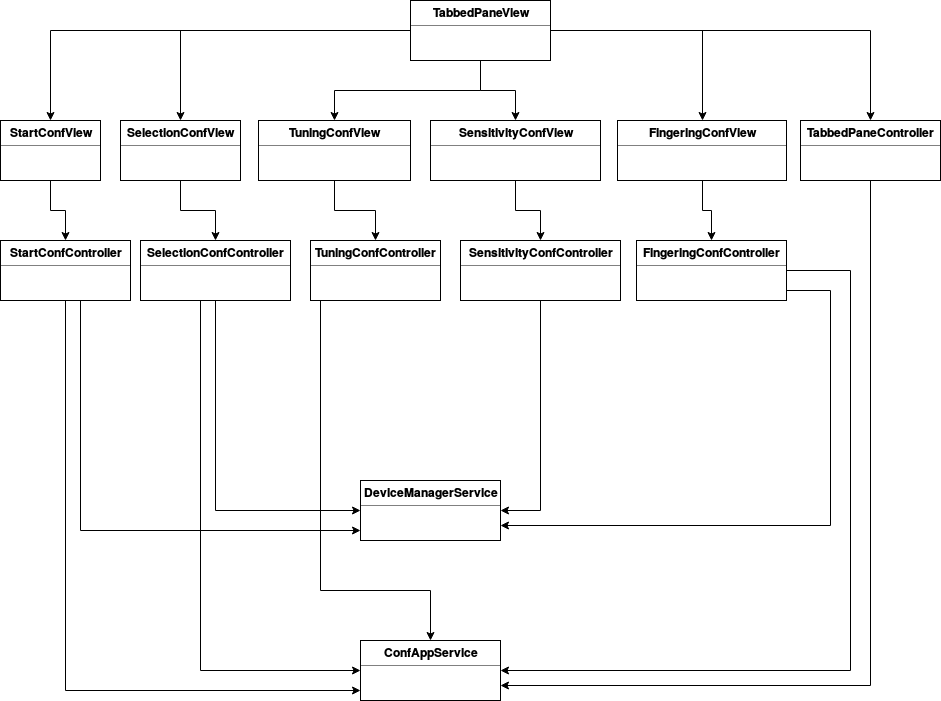
\includegraphics[scale=0.6, angle=90, keepaspectratio=true]{./imagenes/deseno-ni.png}
    % deseno-ni.png: 640x480 pixel, 72dpi, 22.58x16.93 cm, bb=0 0 640 480
    \caption{Deseño de nivel intermedio}
    \label{figura:DesenoNivelIntermedio}
   \end{figure}
   
   Ditos servizos son:
   
   \begin{itemize}
    \item O servizo de dispositivos, encargado de xestionar todo o relacionado
        cos dispositivos hardware en uso: detección, comunicación, etc.
    \item O servizo de configuración, encargado de xestionar todo o relacionado
        coa mesma.
   \end{itemize}
   
   Aplicando BDD e baseándonos na interacción do usuario coas pantallas fóronse
   definindo os distintos casos de uso e a representación conceptual das
   das entidades do modelo para o seu uso polos distintos servizos. \\
   
   A interface do servizo de dispositivos quedou como reflexan as figuras
   \ref{figura:ServizoDispositivos1} a \ref{figura:ServizoDispositivos4}. \\
   
   \begin{figure}[htbp]
    \centering
    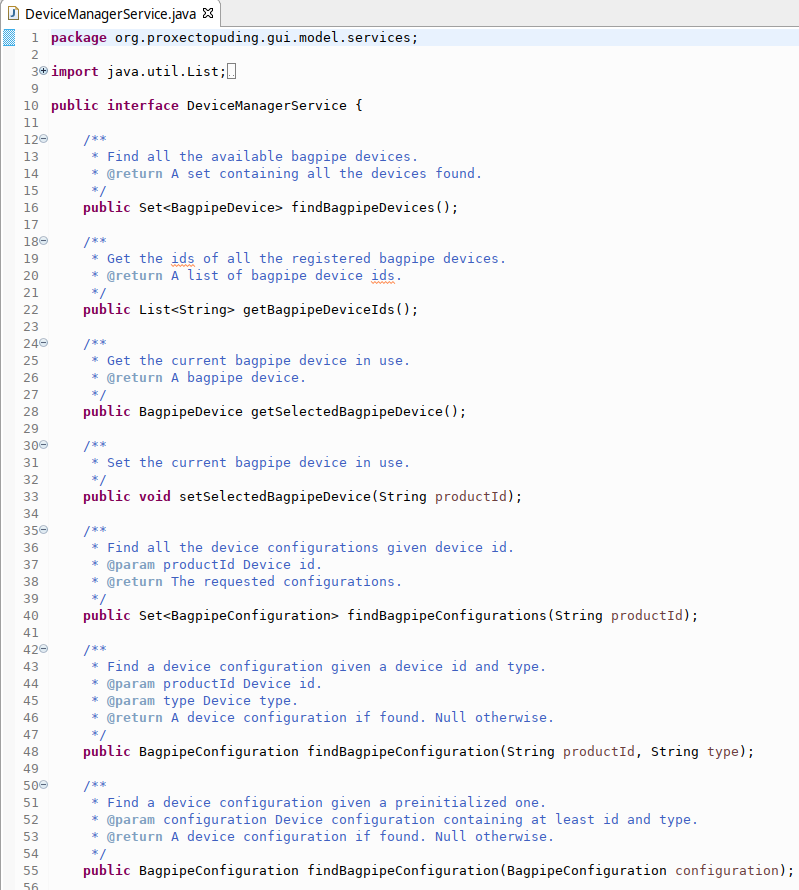
\includegraphics[scale=0.6, keepaspectratio=true]{./imagenes/servizo-dispositivos-1.png}
    % servizo-dispositivos-1.png: 640x480 pixel, 72dpi, 22.58x16.93 cm, bb=0 0 640 480
    \caption{Servizo de dispositivos}
    \label{figura:ServizoDispositivos1}
   \end{figure}
   
   \begin{figure}[htbp]
    \centering
    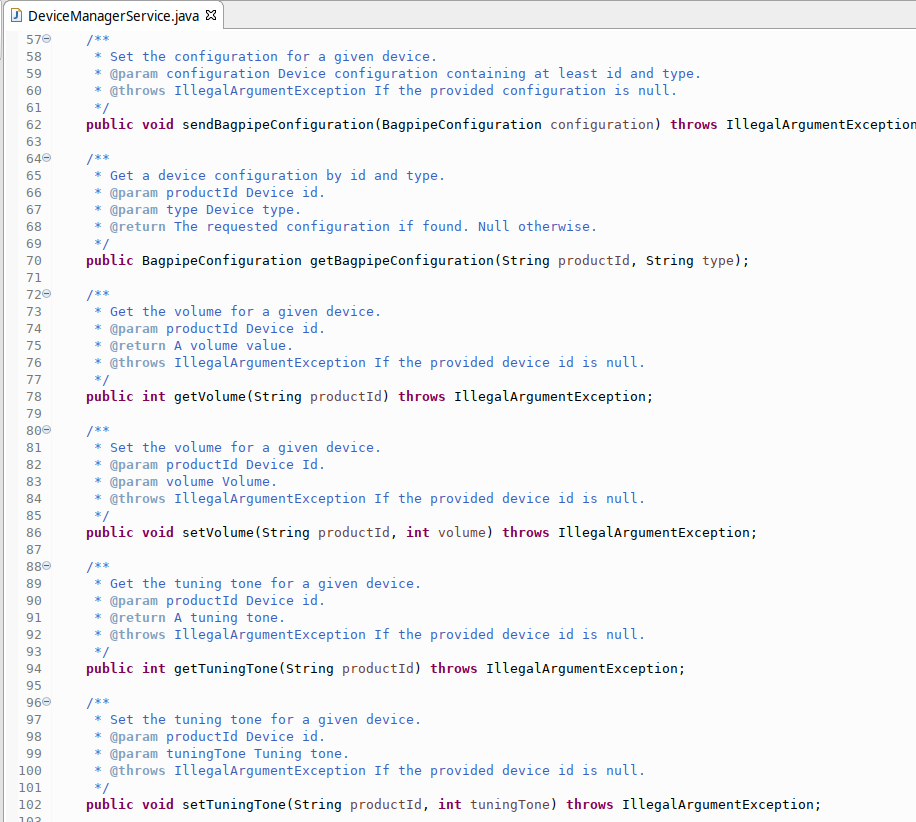
\includegraphics[scale=0.6, keepaspectratio=true]{./imagenes/servizo-dispositivos-2.png}
    % servizo-dispositivos-2.png: 640x480 pixel, 72dpi, 22.58x16.93 cm, bb=0 0 640 480
    \caption{Servizo de dispositivos}
    \label{figura:ServizoDispositivos2}
   \end{figure}
   
   \begin{figure}[htbp]
    \centering
    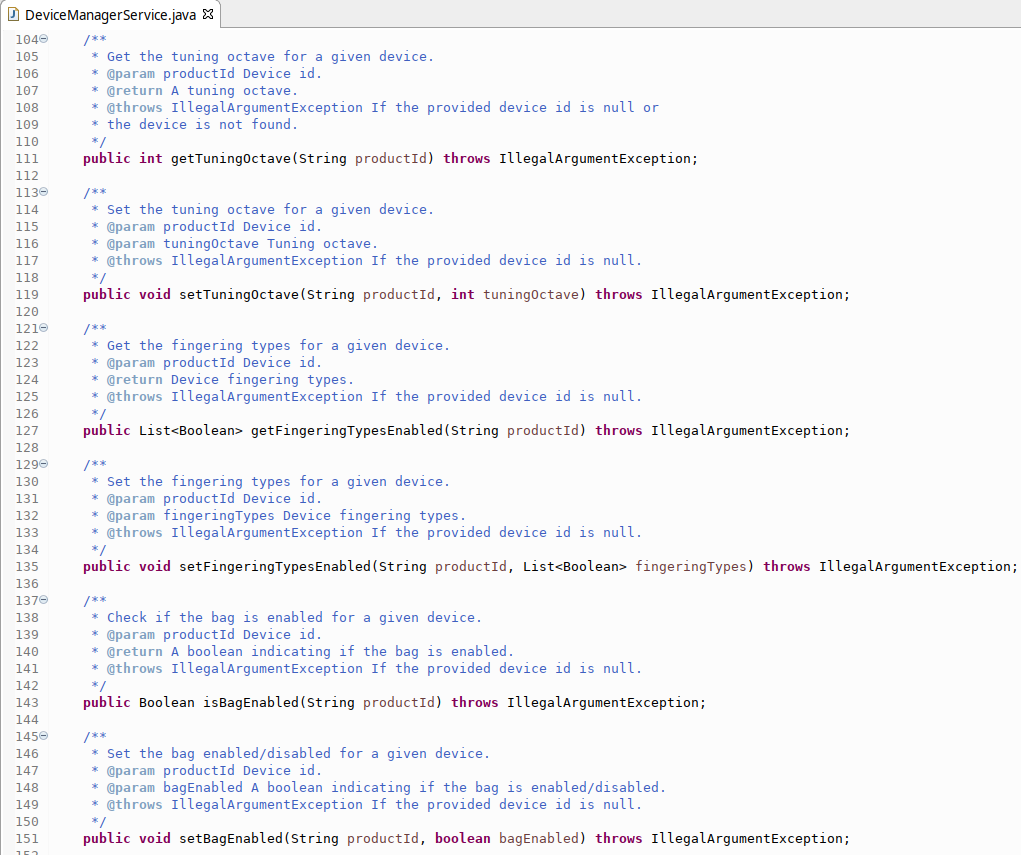
\includegraphics[scale=0.6, keepaspectratio=true]{./imagenes/servizo-dispositivos-3.png}
    % servizo-dispositivos-3.png: 640x480 pixel, 72dpi, 22.58x16.93 cm, bb=0 0 640 480
    \caption{Servizo de dispositivos}
    \label{figura:ServizoDispositivos3}
   \end{figure}
   
   \begin{figure}[htbp]
    \centering
    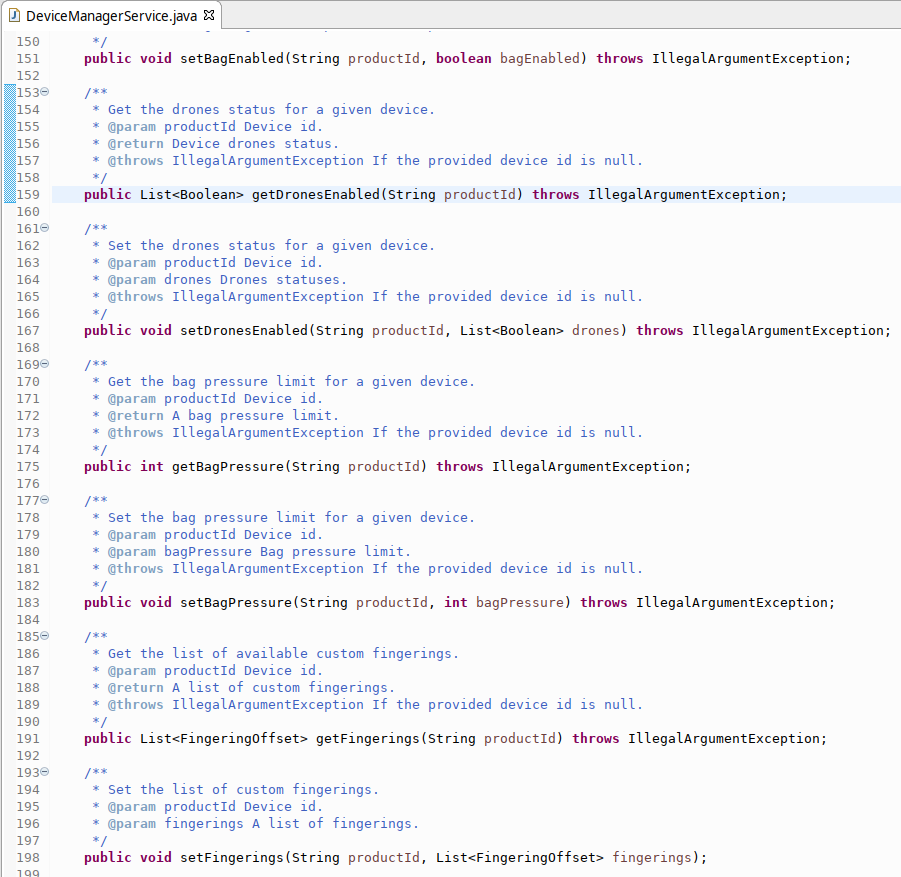
\includegraphics[scale=0.6, keepaspectratio=true]{./imagenes/servizo-dispositivos-4.png}
    % servizo-dispositivo-4s.png: 640x480 pixel, 72dpi, 22.58x16.93 cm, bb=0 0 640 480
    \caption{Servizo de dispositivos}
    \label{figura:ServizoDispositivos4}
   \end{figure}
   
   A interface do servizo de configuración quedou como reflexan as figuras
   \ref{figura:ServizoConfiguracion1} a \ref{figura:ServizoConfiguracion7}. \\
   
   \begin{figure}[htbp]
    \centering
    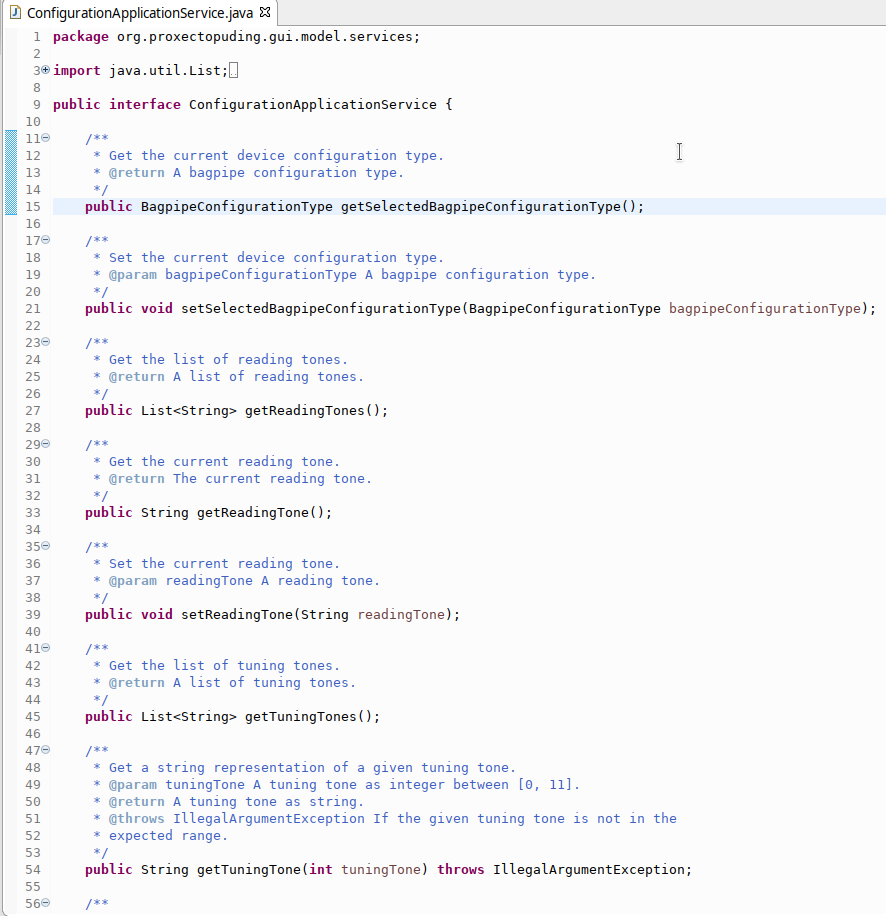
\includegraphics[scale=0.6, keepaspectratio=true]{./imagenes/servizo-configuracion-1.png}
    % servizo-configuracion-1.png: 640x480 pixel, 72dpi, 22.58x16.93 cm, bb=0 0 640 480
    \caption{Servizo de configuración}
    \label{figura:ServizoConfiguracion1}
   \end{figure}
   
   \begin{figure}[htbp]
    \centering
    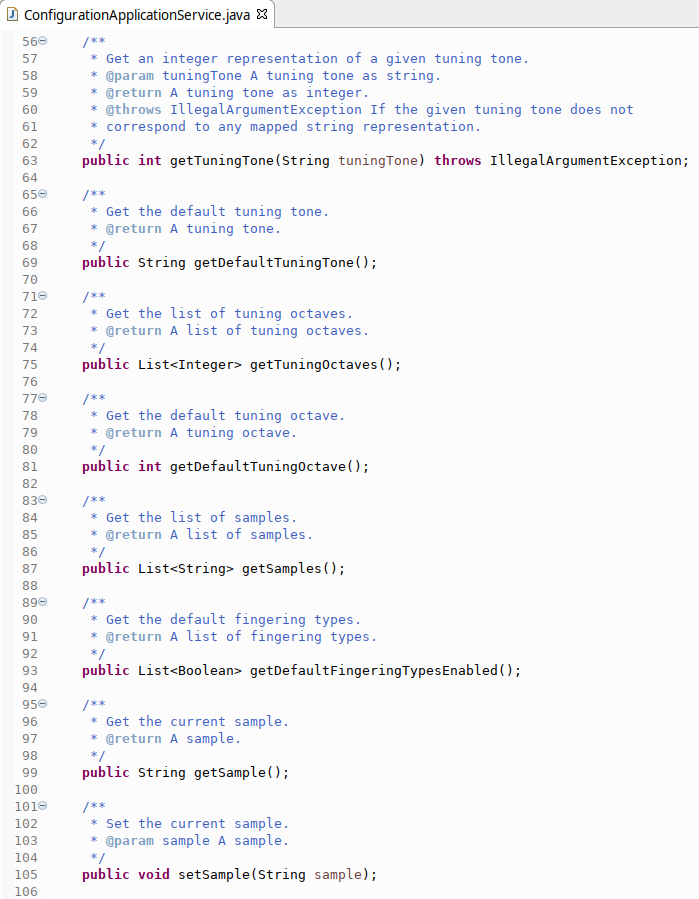
\includegraphics[scale=0.6, keepaspectratio=true]{./imagenes/servizo-configuracion-2.png}
    % servizo-configuracion-2.png: 640x480 pixel, 72dpi, 22.58x16.93 cm, bb=0 0 640 480
    \caption{Servizo de configuración}
    \label{figura:ServizoConfiguracion2}
   \end{figure}
   
   \begin{figure}[htbp]
    \centering
    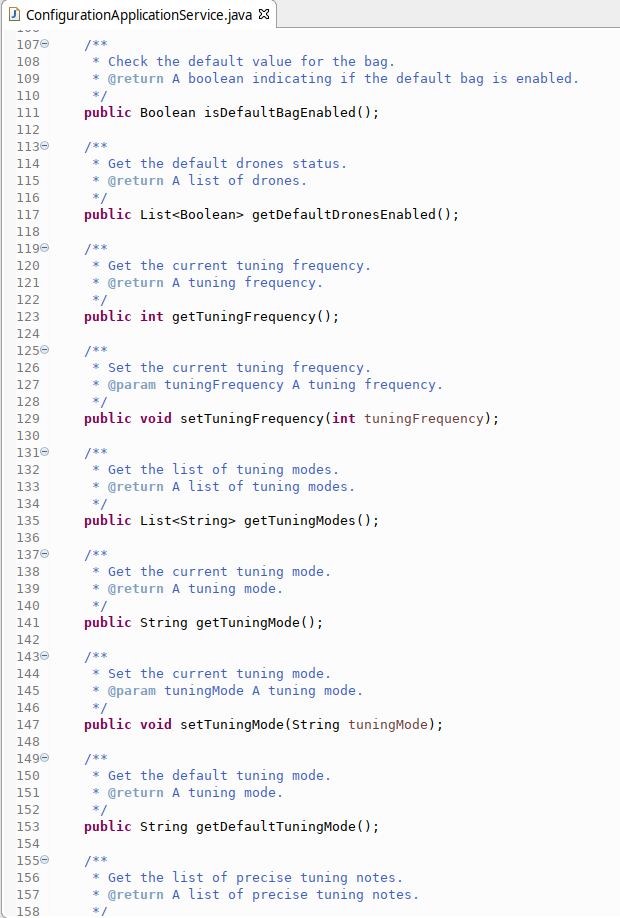
\includegraphics[scale=0.6, keepaspectratio=true]{./imagenes/servizo-configuracion-3.png}
    % servizo-configuracion-3.png: 640x480 pixel, 72dpi, 22.58x16.93 cm, bb=0 0 640 480
    \caption{Servizo de configuración}
    \label{figura:ServizoConfiguracion3}
   \end{figure}
   
   \begin{figure}[htbp]
    \centering
    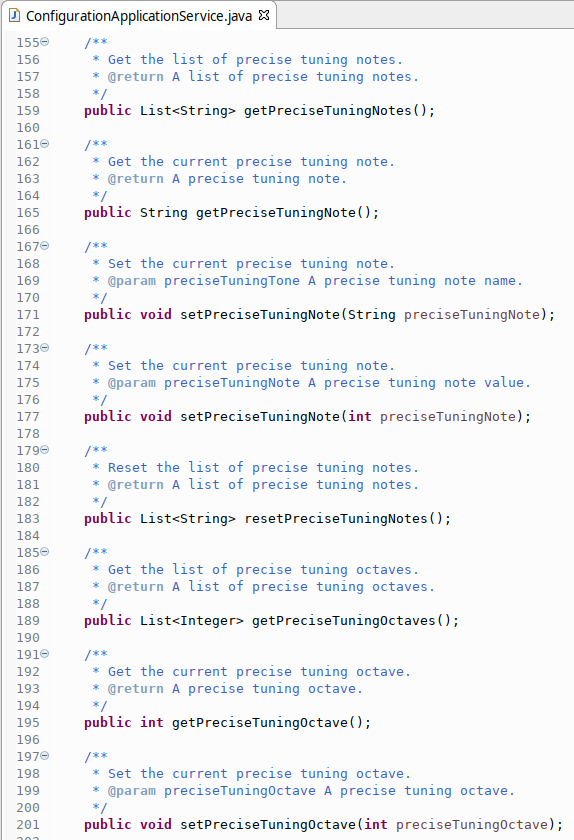
\includegraphics[scale=0.6, keepaspectratio=true]{./imagenes/servizo-configuracion-4.png}
    % servizo-configuracion-4.png: 640x480 pixel, 72dpi, 22.58x16.93 cm, bb=0 0 640 480
    \caption{Servizo de configuración}
    \label{figura:ServizoConfiguracion4}
   \end{figure}
   
   \begin{figure}[htbp]
    \centering
    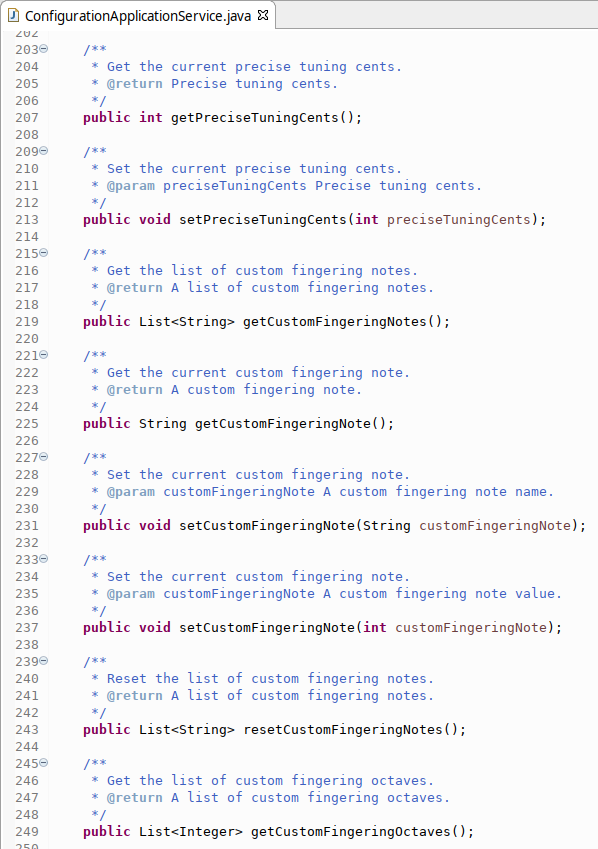
\includegraphics[scale=0.6, keepaspectratio=true]{./imagenes/servizo-configuracion-5.png}
    % servizo-configuracion-5.png: 640x480 pixel, 72dpi, 22.58x16.93 cm, bb=0 0 640 480
    \caption{Servizo de configuración}
    \label{figura:ServizoConfiguracion5}
   \end{figure}
   
   \begin{figure}[htbp]
    \centering
    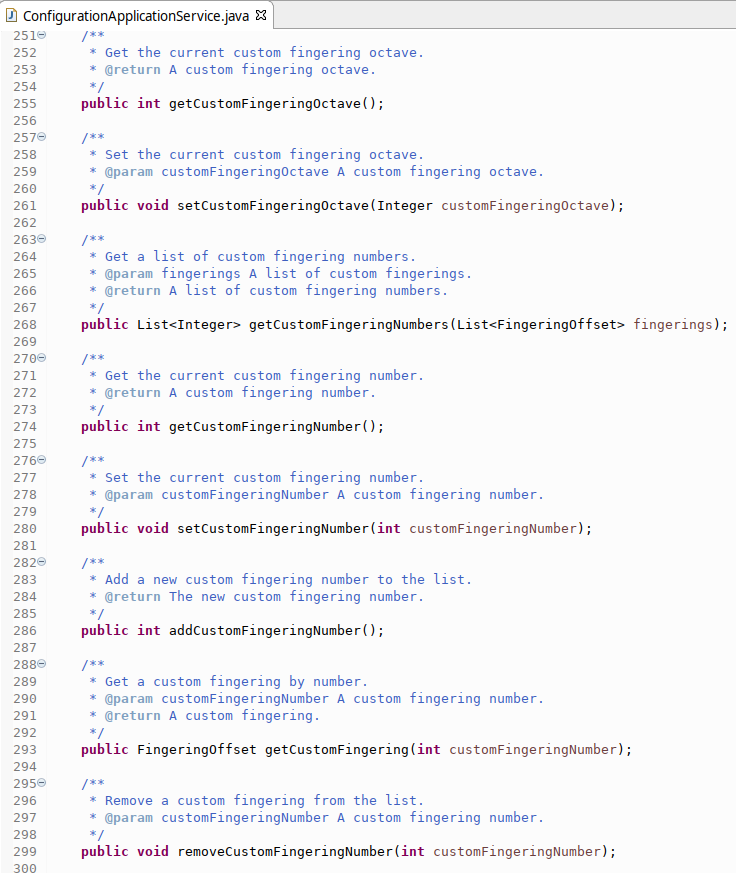
\includegraphics[scale=0.6, keepaspectratio=true]{./imagenes/servizo-configuracion-6.png}
    % servizo-configuracion-6.png: 640x480 pixel, 72dpi, 22.58x16.93 cm, bb=0 0 640 480
    \caption{Servizo de configuración}
    \label{figura:ServizoConfiguracion6}
   \end{figure}
   
   \begin{figure}[htbp]
    \centering
    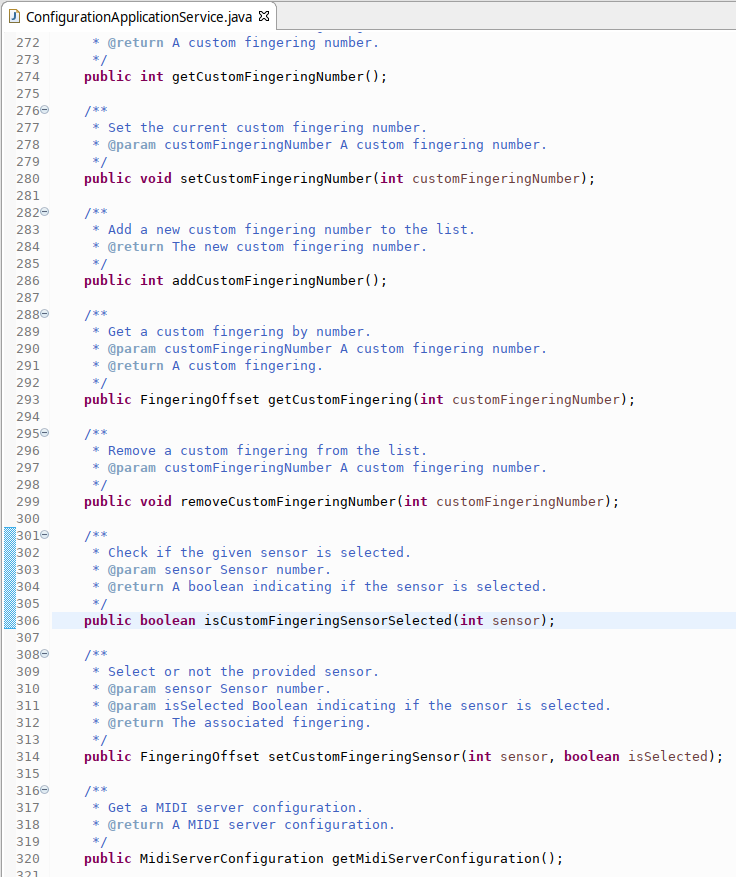
\includegraphics[scale=0.6, keepaspectratio=true]{./imagenes/servizo-configuracion-7.png}
    % servizo-configuracion71.png: 640x480 pixel, 72dpi, 22.58x16.93 cm, bb=0 0 640 480
    \caption{Servizo de configuración}
    \label{figura:ServizoConfiguracion7}
   \end{figure}
   
   Como se pode apreciar nas interfaces dos servizos, as principais entidades
   resultantes do modelo son o dispositivo, os distintos tipos de configuración
   do mesmo e o servidor MIDI, que quedarían como amosan as figuras 
   \ref{figura:BagpipeDevice} a \ref{figura:MidiServerConfiguration}. \\
   
   \begin{figure}[htbp]
    \centering
    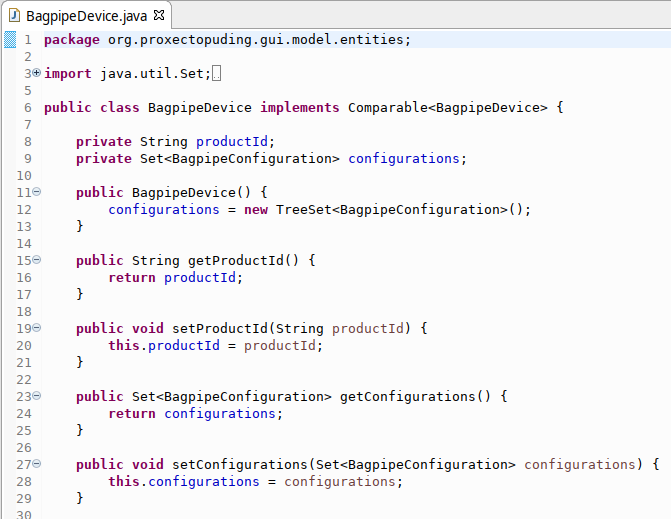
\includegraphics[scale=0.6, keepaspectratio=true]{./imagenes/bagpipe-device.png}
    % bagpipe-device.png: 640x480 pixel, 72dpi, 22.58x16.93 cm, bb=0 0 640 480
    \caption{Dispositivo}
    \label{figura:BagpipeDevice}
   \end{figure}
   
   \begin{figure}[htbp]
    \centering
    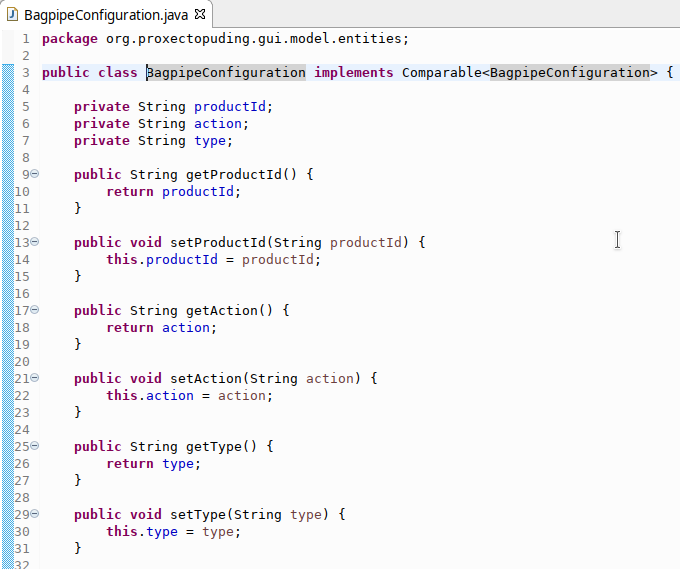
\includegraphics[scale=0.6, keepaspectratio=true]{./imagenes/bagpipe-configuration.png}
    % bagpipe-configuration.png: 640x480 pixel, 72dpi, 22.58x16.93 cm, bb=0 0 640 480
    \caption{Configuración}
    \label{figura:BagpipeConfiguration}
   \end{figure}
   
   \begin{figure}[htbp]
    \centering
    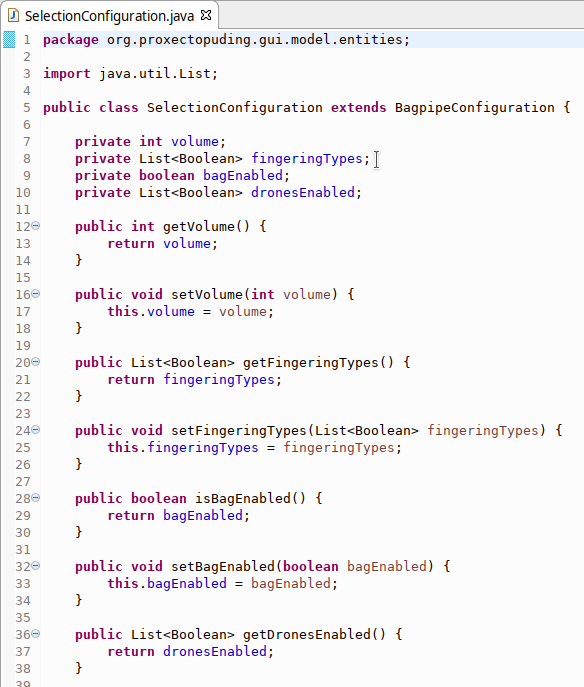
\includegraphics[scale=0.6, keepaspectratio=true]{./imagenes/selection-configuration.png}
    % selection-configuration.png: 640x480 pixel, 72dpi, 22.58x16.93 cm, bb=0 0 640 480
    \caption{Configuración de selección}
    \label{figura:SelectionConfiguration}
   \end{figure}
   
   \begin{figure}[htbp]
    \centering
    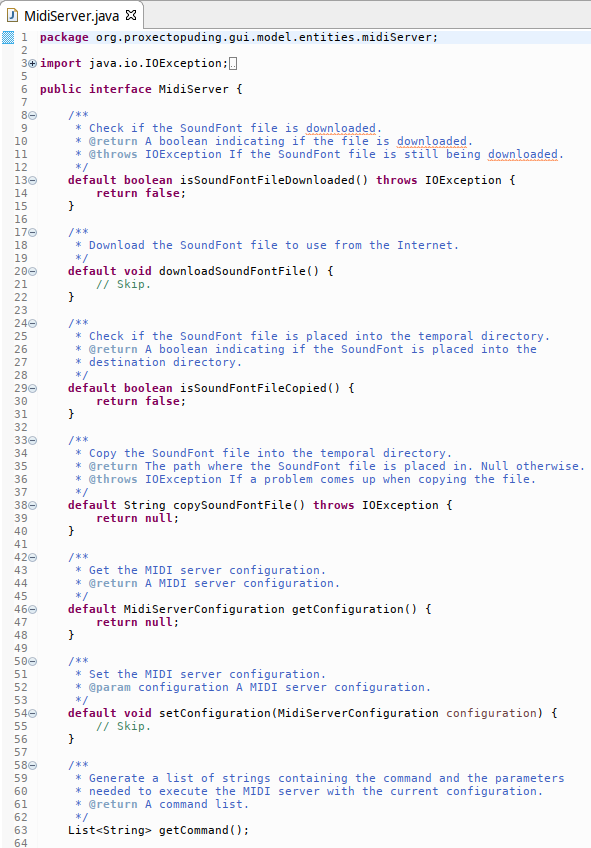
\includegraphics[scale=0.6, keepaspectratio=true]{./imagenes/midi-server.png}
    % midi-server.png: 640x480 pixel, 72dpi, 22.58x16.93 cm, bb=0 0 640 480
    \caption{Servidor MIDI}
    \label{figura:MidiServer}
   \end{figure}
   
   \begin{figure}[htbp]
    \centering
    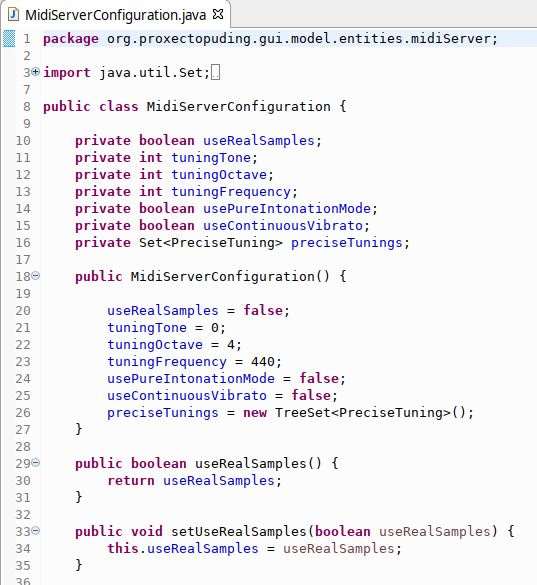
\includegraphics[scale=0.6, keepaspectratio=true]{./imagenes/midi-server-configuration.png}
    % midi-server-configuration.png: 640x480 pixel, 72dpi, 22.58x16.93 cm, bb=0 0 640 480
    \caption{Configuración do servidor MIDI}
    \label{figura:MidiServerConfiguration}
   \end{figure}
   
   Definidos xa servizos e entidades do modelo, procedeuse a conectar vista e
   modelo a través do controlador, tal e como se indica no UML. Desta maneira
   comprobamos de maneira práctica se encaixaban ven ambas partes e se non
   esqueciamos nada importante que puidese implicar un retraballo severo de
   dectectarse nunha fase posterior.

   \paragraph{Gravación das mostras}
   
   Debido á cantidade de horas a invertir neste apartado, entre a gravación das
   mostras e a xeración da fonte de son e á dispoñibilidade de outras fontes xa
   dispoñibles públicamente, aínda que de menor calidade, decidiuse adiar este
   apartado a unha fase posterior dada a pouca relevancia académica do mesmo e
   invertir ditas horas en apartados de maior calado.

\section{Desenvolvemento e validación do seguinte nivel do producto}

 \subsection{Simulacións, modelos e programas de proba}
 
 As probas realizadas neste nivel do producto consistiron inicialmente en
 realizar as mesmas probas da fase anterior sobre os novos prototipos para
 verificar que a implementación cumpría coa especificación de requisitos e de
 que non pasabamos nada por alto. \\
 
 Posteriormente, de maneira máis formal e seguindo a metodoloxía de
 desenvolvemento citada (BDD/TDD), definíronse unha serie de probas funcionais
 a nivel de unidade, integración e aceptación a nivel de servizos e para ambos
 sistemas, de maneira que se puidesen validar e verificar o seu funcionamento
 tanto antes coma despois de implementar a lóxica do mesmos. Ditas probas serán
 explicadas en detalle ó final deste capítulo. \\

 \subsection{Deseño detallado}

  \subsubsection{Deseño hardware}
  
  Contando xa cun deseño formal e detallado do producto hardware dende fases
  anteriores e non tendo detectado novos problemas, decidimos seguir empregando
  o \textit{Prototipo 3 hardware} (figura \ref{figura:Prototipo3HardwareBB1})
  coma deseño do mesmo.

  \subsubsection{Deseño software}
  
  Baseándose no deseño de nivel medio do prototipo software operacional
  (figura \ref{figura:DesenoNivelIntermedio}) e nas carencias e melloras
  detectadas durante as probas realizadas sobre a implementación de dito
  prototipo, chegouse a un deseño de nivel medio máis detallado onde se
  incluíron novos servizos que agrupan funcionalidades relacionadas que ven non
  estaban reflexadas de maneira explícita ou teñen un peso máis secundario. \\
  
  Na figura \ref{figura:DesenoBaixoNivel} pode apreciarse o diagrama UML deste
  deseño máis completo.
  
  \begin{figure}[htbp]
    \centering
    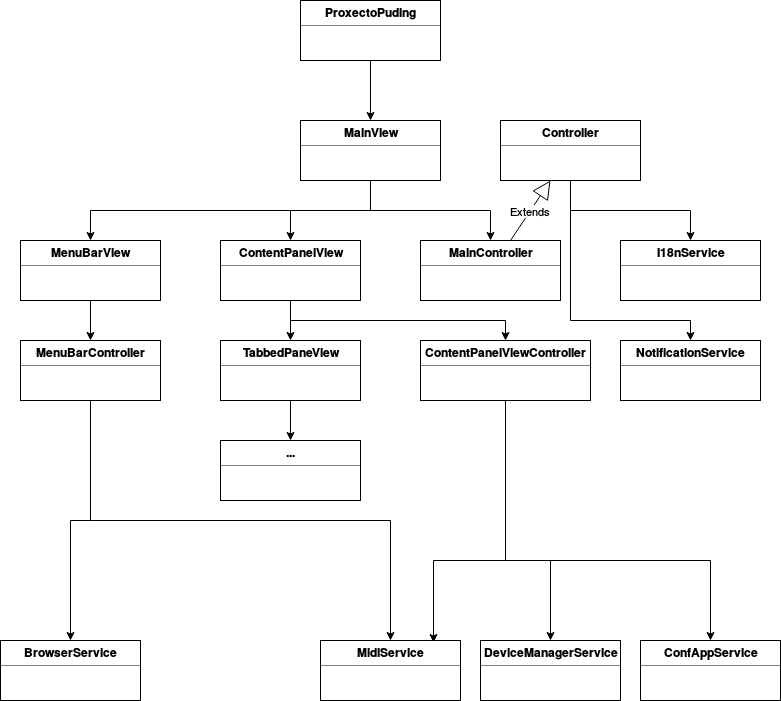
\includegraphics[scale=0.6, keepaspectratio=true]{./imagenes/deseno-bn.png}
    % deseno-bn.png: 640x480 pixel, 72dpi, 22.58x16.93 cm, bb=0 0 640 480
    \caption{Deseño detallado}
    \label{figura:DesenoBaixoNivel}
   \end{figure}
  
  Entre ditos servizos figuran:
   
   \begin{itemize}
    \item O servizo de internacionalización, encargado de proporcionar as
        mensaxes da aplicación no idioma do usuario.
    \item O servizo de notificacións, encargado de xestionar a comunciación
        entre as distintas partes da interface mediante eventos.
    \item O servizo de navegación web, que permite xestionar a apertura da
        documentación da aplicación directamente no navegador do sistema.
    \item O servizo MIDI, que se encarga de xestionar todo o relacionado coas
        operacións sobre o servidor MIDI.
   \end{itemize}
   
   Aplicando BDD e baseándonos na interacción do usuario coas pantallas fóronse
   definindo os distintos casos de uso e a representación conceptual das
   das entidades do modelo para o seu uso polos distintos servizos. \\
   
   A interfaces dos distintos servizos quedaron tal e como reflexan as figuras
   \ref{figura:ServizoI18n} a \ref{figura:ServizoMidi}. \\
   
   \begin{figure}[htbp]
    \centering
    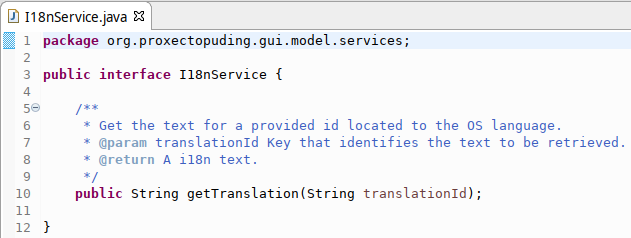
\includegraphics[scale=0.6, keepaspectratio=true]{./imagenes/servizo-i18n.png}
    % servizo-i18n.png: 640x480 pixel, 72dpi, 22.58x16.93 cm, bb=0 0 640 480
    \caption{Servizo de internacionalización}
    \label{figura:ServizoI18n}
   \end{figure}
   
   \begin{figure}[htbp]
    \centering
    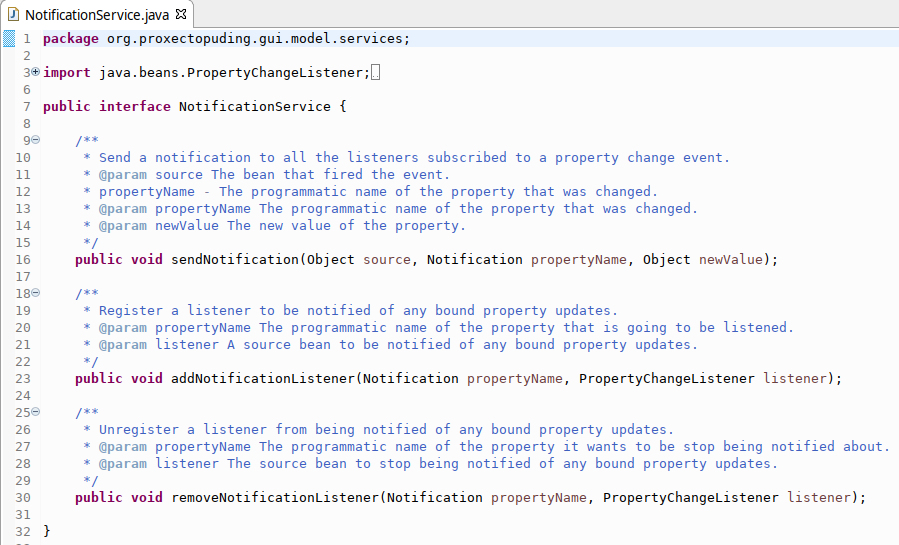
\includegraphics[scale=0.6, keepaspectratio=true]{./imagenes/servizo-notificacions.png}
    % servizo-notificacions.png: 640x480 pixel, 72dpi, 22.58x16.93 cm, bb=0 0 640 480
    \caption{Servizo de notificacións}
    \label{figura:ServizoNotificacions}
   \end{figure}
   
   \begin{figure}[htbp]
    \centering
    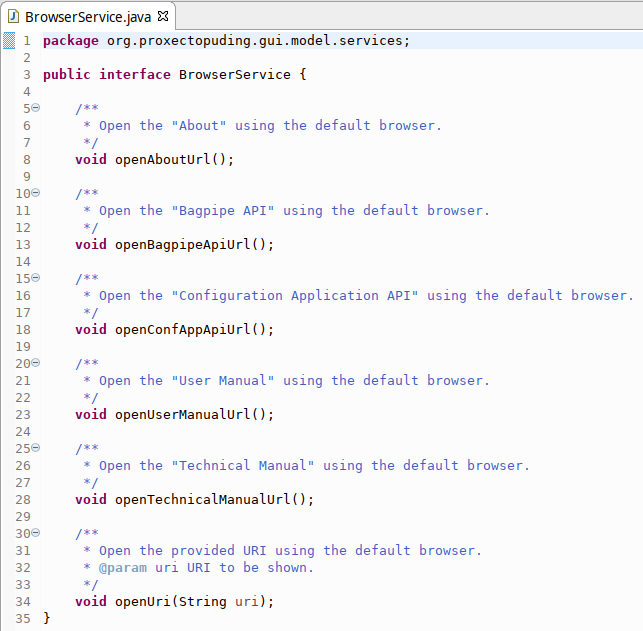
\includegraphics[scale=0.6, keepaspectratio=true]{./imagenes/servizo-navegacion.png}
    % servizo-navegacion.png: 640x480 pixel, 72dpi, 22.58x16.93 cm, bb=0 0 640 480
    \caption{Servizo de navegación web}
    \label{figura:ServizoNavegacion}
   \end{figure}
   
   \begin{figure}[htbp]
    \centering
    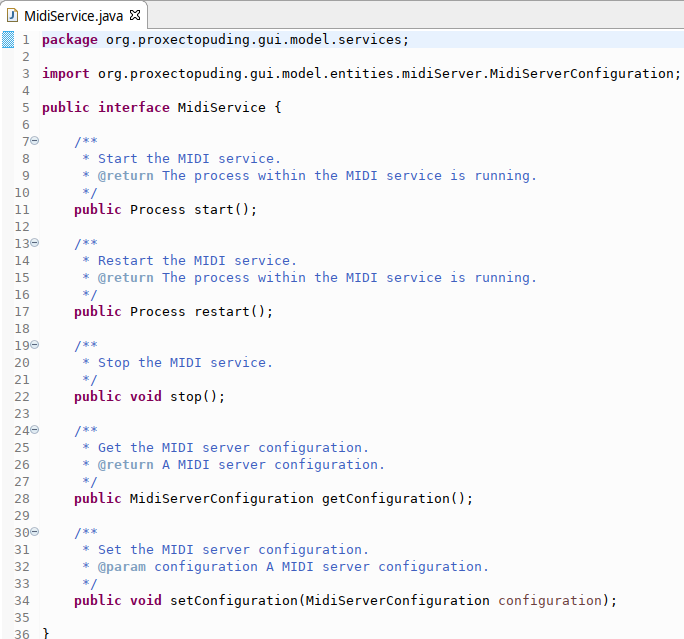
\includegraphics[scale=0.6, keepaspectratio=true]{./imagenes/servizo-midi.png}
    % servizo-midi.png: 640x480 pixel, 72dpi, 22.58x16.93 cm, bb=0 0 640 480
    \caption{Servizo MIDI}
    \label{figura:ServizoMidi}
   \end{figure}
   
   Redefinidos xa servizos e entidades do modelo, procedeuse a reconectar vista
   e modelo a través do controlador facendo uso dos mesmos, tal e como se indica
   no UML. Desta maneira recomprobamos de maneira práctica se encaixaban ven
   ambas partes e se non esqueciamos nada importante que puidese implicar un
   retraballo severo de dectectarse nunha fase posterior.

 \subsection{Ensamblado e codificación}

  \subsubsection{Ensamblado}
  
  Debido a unha serie de razóns de peso (detallados na sección de incidencias),
  descartouse a integración completa e ensamblado de todo o hardware nunha única
  montaxe:
  
  \begin{itemize}
    \item Con respecto á integración, durante a fase final de codificación
        e integración software xurdiron unha serie de problemas que simplemente
        aconsellaron non acoplar todos os compoñentes na mesma montaxe.
    \item Con respecto ó encapsulado, ó non ter toda a montaxe integrada, perde
        a súa razón de ser, ademáis de ser contraproducente mentres non se
        rematen as probas, tal e como se comentou antes. Este sería o paso final
        en calquera caso.
   \end{itemize}

  \subsubsection{Codificación}
  
  Como se comentou con anterioridade, debido á metodoloxía empregada (BDD/TDD),
  a codificación tanto do firmware coma da aplicación de configuración foi o
  último paso de todos, dado que primeiramente se definiron as probas. \\
  
  Unha vez tivemos definidas as probas, para o que fomos en sentido
  \textit{top-down} ata o nivel de servizo, cambiamos o sentido a
  \textit{bottom-up} para facer a implementación dos mesmos en ámbolos casos.
  
   \paragraph{Hardware}
   
   A codificación do firmware do hardware levouse a cabo por partes e de menor
   a maior dificultade:
   
   \begin{itemize}
    \item Sensor de presión.
    \item Sensores capacitivos.
    \item Lector de tarxetas.
    \item Receptor: configuración e reproducción MIDI.
   \end{itemize}
   
   Aínda que a maior dificultade común a todas elas foi a complexidade da
   documentación e a falta dun entorno de desenvolvemento serio. \\
   
   Comezando polo \textbf{sensor de presión}, este caso é a excepción que 
   confirma a regra. Ó ser unha peza desenvolvida por Bosh (compañía moi seria
   en canto a desenvolvemento de sensores), a folla de especificacións
   \cite{Bmp085DataSheet} é impecable. \\
   
    O proceso consistiu en:
    
    \begin{itemize}
    \item Solicitar a lectura da presión.
    \item Definir e ler os rexistros da ROM onde se almacenan os coeficientes de
        calibración do disposito.
    \item Definir e ler os rexistros da ROM onde se almacenan os coeficientes de
        calibración do disposito.
    \item Ler a temperatura sen compensar (4.5 ms).
    \item Definir o modo de lectura da presión e ler a presión sen compensar.
        Como nos interesaba a velocidade e o baixo consumo máis que a precisión,
        optouse polo modo de ultra baixo consumo (4.5 ms), co que se obteñen
        valores bastante desviados, pero como o que precisamos a nivel de lóxica
        de negocio é un valor umbral (ou dous se optamos por un comparador con
        histérese), que o valor sexa máis ou menos real non é o importante.
    \item Calcular a temperatura real aplicando os coeficientes de calibración.
    \item Calcular a presión real aplicando os coeficientes de calibración.
    \item Devolver a presión real, que é o valor que realmente nos interesa,
        invertindo un tempo de arredor de 9 ms, que está por debaixo dos 100 ms
        que se adoitan considerar como tempo real duro para intrumentación MIDI
        e incluso por debaixo dos 10 ms que se considera o óptimo e que serían
        imperceptibles.
   \end{itemize}
   
   Dado que tanto as direccións dos rexistros dos coeficientes de calibración e
   a aplicación dos mesmos e o pseudo-código especificado
   \ref{figura:Bmp085PseudoCodigo} estaban moi ben explicados, foi relativamente
   sinxelo facer funcionar o sensor e que pasase as probas definidas
   anteriormente. Os resultados das mesmas comentaranse no apartado de probas
   unitarias. \\
   
   Finalmente, entre documentación, código e probas, obtivemos un módulo de moi
   baixo nivel en C de arredor de 500 líneas. \\
   
   \begin{figure}[htbp]
    \centering
    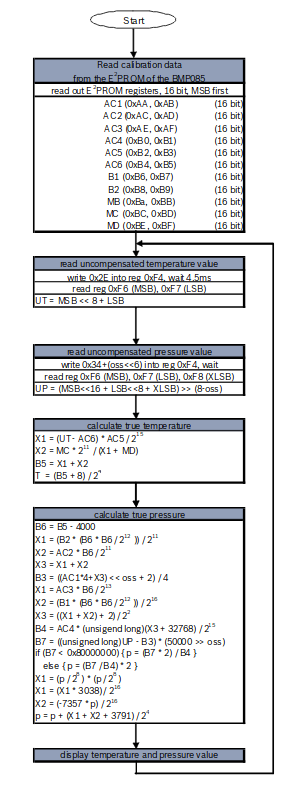
\includegraphics[scale=0.6, keepaspectratio=true]{./imagenes/bmp085-pseudocodigo.png}
    % servizo-midi.png: 640x480 pixel, 72dpi, 22.58x16.93 cm, bb=0 0 640 480
    \caption{Pseudo-código do sensor de presión}
    \label{figura:Bmp085PseudoCodigo}
   \end{figure}
   
   Continuando polos \textbf{sensores capacitivos}, a folla de especificacións
   \cite{MPR121}, de Freescale neste caso, tamén é de calidade, polo que
   facilitou o desenvolvemento. \\
   
   O proceso consistiu en:
    
    \begin{itemize}
    \item Solicitar a lectura da presión mediante I2C.
    \item Definir e ler os rexistros da ROM onde se almacenan as configuracións
        e e valores medidos do disposito.
    \item Ler os valores dos sensores.
    \item Devolver os valores medidos.
   \end{itemize}
   
   A configuración dos rexistros foi de lonxe a parte máis complexa e tediosa.
   Houbo que configurar medio cento de rexistros agrupados nunha decena de
   grupos funcionais e facelo nunha orde concreta, antes de poder facer calquera
   outra operación. \\
   
   En xeral, precisamos obter o valor dos 9 bits/sensores menos significativos
   da placa (que empregaremos para as dixitacións), máis o 13º, sensor virtual
   de presencia (que empregaremos para o vibrato). \\
   
   A lectura dos valores dos sensores realízase primeiro en bruto, sendo pasados
   a continuación por tres filtros de distinto tipo, como se pode apreciar na
   figura \ref{figura:Mpr121Medicion}. \\
   
   \begin{figure}[htbp]
    \centering
    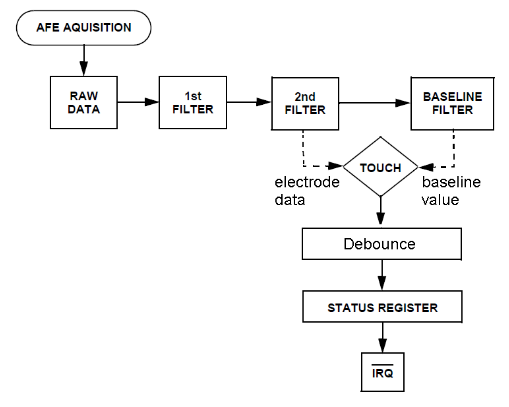
\includegraphics[scale=0.6, keepaspectratio=true]{./imagenes/mpr121-medicion.png}
    % mpr121-medicion.png: 640x480 pixel, 72dpi, 22.58x16.93 cm, bb=0 0 640 480
    \caption{Medición dos sensores capacitivos}
    \label{figura:Mpr121Medicion}
   \end{figure}
   
   O sensor de proximidade é un sensor virtual que calcula o seu valor en
   función do valor dos outros 12 sensores físicos, de maneira que podemos
   empregalo para calcular pequenas variacións ou vibracións dos son en función
   de se hai outros dedos próximos ós sensores que non están sendo empregados
   na dixitación. \\
   
   Outro punto moi importante que descubrimos na folla de especificacións é que
   os sensores son auto-calibrables, polo que o requisito sobre o axuste da
   sensibilidade do sensores, logo de facer probas con distinta xente e vendo
   que os valores eran correctos, quedou cuberto pola parte hardware sen
   necesidade de cubrilo dende o software de configuración, motivo polo que se
   revisou a pantalla de configuración da sensibilidade do punteiro, eliminando
   a sección de configuración da sensibilidade dos sensores e quedando como se
   amosa na figura \ref{figura:ConfiguracionSensibilidade}. \\
   
   \begin{figure}[htbp]
    \centering
    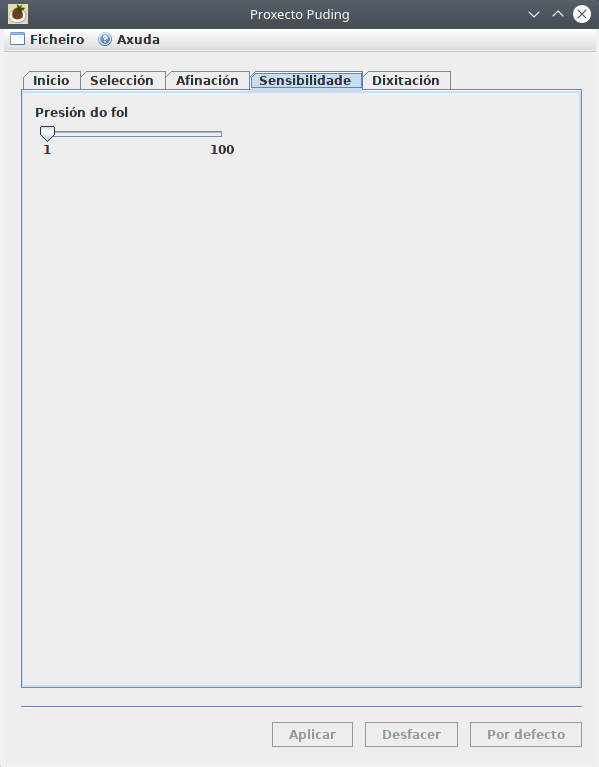
\includegraphics[scale=0.6, keepaspectratio=true]{./imagenes/configuracion-sensibilidade.png}
    % configuracion-sensibilidade.png: 640x480 pixel, 72dpi, 22.58x16.93 cm, bb=0 0 640 480
    \caption{Configuración da sensibilidade do punteiro}
    \label{figura:ConfiguracionSensibilidade}
   \end{figure}
   
   Feitos funcionar os sensores e que pasasen as probas definidas anteriormente,
   os resultados das mesmas comentaranse no apartado de probas unitarias. \\
   
   Finalmente, entre documentación, código e probas, obtivemos un módulo de moi
   baixo nivel en C de arredor de 500 líneas. \\
   
   Seguindo polo \textbf{lector de tarxetas}, a documentación proporcionada por
   4D Systems \cite{MicroDriveG1} é claramente escasa e incompleta. En xeral,
   especifica relativamente ben os casos \textit{happy path}, ou o camiño
   típico, pero en moitos casos non especifica qué pasa en caso de erro ou a
   descrición resulta ambigua, casos que cando falamos de hardware, son custosos
   cando non imposibles de reproducir de maneira forzada, o cal dificulta unha
   implementación completa e correcta do firmware. \\
   
   O proceso consistiu en:
    
   \begin{itemize}
    \item Inicializar a comunicación por porto serie.
    \item Esperar a que o dispositivo arrinque (500 ms).
    \item Esperar a que o dispositivo detecte a velocidade do porto serie.
    \item Ler ou escribir información na tarxeta de memoria.
   \end{itemize}
   
   A complexidade deste módulo residiu principalmente na incertidume na que nos
   movemos todo o rato debido á falta de documentación, que nos obrigou a estar
   probando cada pequeno paso que dabamos e a tomar decisións un pouco drásticas
   para cubrirnos en saúde. \\
   
   Basicamente, as operacións que precisamos principalmente de todas as
   dispoñibles, serían as de lectura e escritura dun ficheiro. \\
   
   Como exemplo, a documentación di que se poden ler/escribir datos en bloques
   de 1 a 50/100 bytes (con/sen ACK), pero non indica en ningún momento qué pasa
   co último bloque se o tamaño total non é múltiplo do tamaño de bloque. \\
   
   Neste caso concreto, por exemplo, optamos pola opción máis segura pero menos
   eficiente de todas: ACKs por bloques de 1 byte. Como o tamaño dos ficheiros
   é de poucos centos de bytes, a penalización apenas é perceptible. \\
   
   % TODO Revisar este punto despois de pasar as probas.
   
   Feita funcionar a lectura/escritura de ficheiros e que pasasen as probas
   definidas anteriormente, os resultados das mesmas comentaranse no apartado de
   probas unitarias. \\
   
   Finalmente, entre documentación, código e probas, obtivemos un módulo de moi
   baixo nivel en C de arredor de 700 líneas. \\
   
   E rematando polo \textbf{receptor}, que á súa vez se divide entre a lóxica
   de configuración e a de reproducción. \\
   
   Feitos funcionar os outros módulos, era o momento de implementar a lóxica de
   negocio da capa inmediatamente superior, é dicir, a do receptor, onde se
   empregrarían o módulo do lector de tarxetas para a configuración e os módulos
   de presión e capacitivos para a reproducción. \\
   
   % TODO Pendente de redactar.
   
   Finalmente, entre documentación, código e probas, obtivemos un módulo de
   baixo nivel en C de arredor de 1100 líneas.
   
   \paragraph{Software}

 \subsection{Probas de unidade}

 \subsection{Integración e probas}

 \subsection{Probas de aceptación}

 \subsection{Implantación}
